\newpage
\subsection{QuizziPedia::Front-End::Controllers}


\begin{figure} [ht]
	\centering
	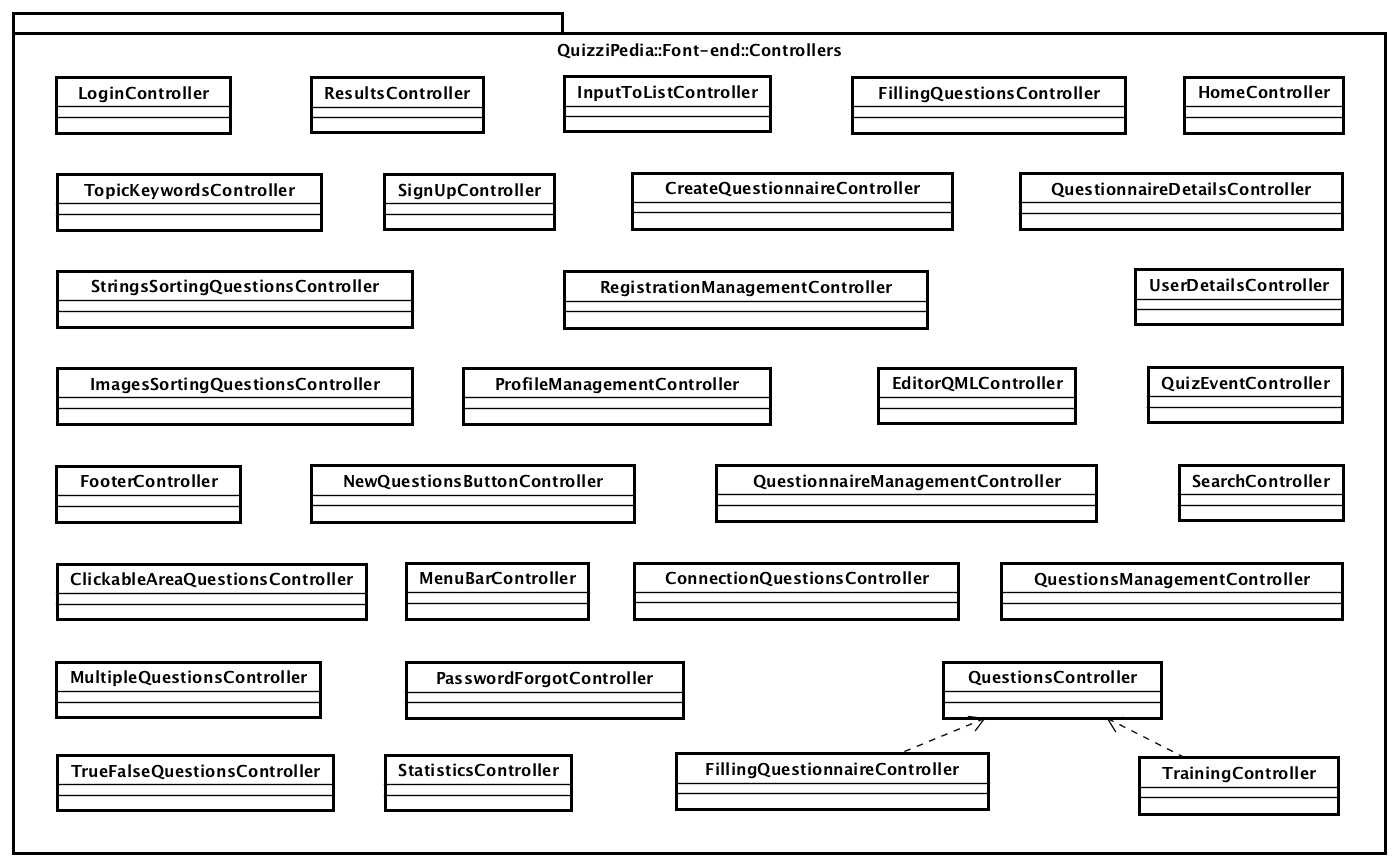
\includegraphics[scale=0.45]{UML/Package/QuizziPedia_Front-End_Controllers.png}
	\caption{QuizziPedia::Front-End::Controllers}
\end{figure} \FloatBarrier

\subsubsection{Informazioni generali}
\begin{itemize}
	\item \textbf{Descrizione}: package che contiene i controller individuati per la parte front-end dell'applicazione;
	\item \textbf{Padre}: \texttt{Front-End};
	\item \textbf{Interazione con altri componenti}:
	\begin{itemize}
		\item \texttt{Models}: package che contiene le classi model individuate;
		\item \texttt{Services}: package che contiene le classi services individuate.
	\end{itemize} 
\end{itemize}
\subsubsection{Classi}

\paragraph{QuizziPedia::Front-End::Controllers::LoginController}
\begin{figure} [ht]
	\centering
	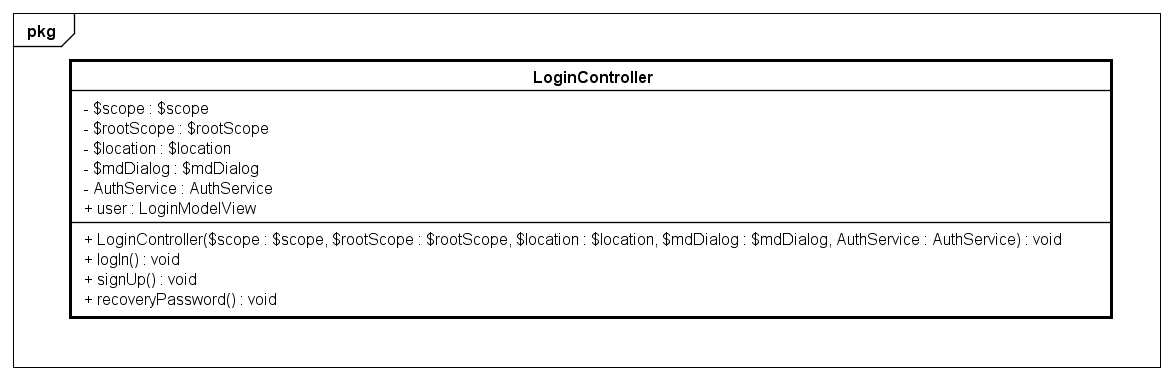
\includegraphics[scale=0.45]{UML/Classi/Front-End/QuizziPedia_Front-end_Controller_LoginController.png}
	\caption{QuizziPedia::Front-End::Controllers::LoginController}
\end{figure} \FloatBarrier
\begin{itemize}
	\item \textbf{Descrizione}: questa classe permette di gestire l'autenticazione dell'utente al sistema; 
	\item \textbf{Utilizzo}: fornisce le funzionalità di autenticazione al sistema, compresa la gestione di situazioni di errore di autenticazione;
	\item \textbf{Relazione con altre classi}:
	\begin{itemize}
		\item \textit{IN} \texttt{LoginModelView}: classe di tipo modelview la cui istanzazione è contenuta all'interno della variabile di ambiente \$scope di \textit{Angular.js\ped{G}}. All'interno di essa sono presenti le variabili e i metodi necessari per il \textit{Two-Way Data-Binding\ped{G}} tra la view \texttt{LoginView} e il controller \texttt{LoginController};
		\item \textit{IN} \texttt{AuthService}: questa classe permette di gestire la registrazione e l'autenticazione di un utente;
	\end{itemize}
	\item \textbf{Attributi}:
	\begin{itemize}
		\item \texttt{-} \texttt{\$scope: \$scope} \\
		Campo dati contenente un riferimento all’oggetto \$scope creato da \textit{Angular\ped{G}}. Viene utilizzato come mezzo di comunicazione tra il controller e la view. Contiene gli oggetti che definiscono il viewmodel e il model dell’applicazione;
		\item \texttt{-} \texttt{\$location: \$location} \\
		Campo dati contenente un riferimento al servizio creato da \textit{Angular\ped{G}} che permette di accedere alla barra degli indirizzi del \textit{browser\ped{G}}, i cambiamenti all’URL nella barra degli indirizzi si riflettono in questo oggetto e viceversa;
		\item \texttt{-} \texttt{\$mdDialog: \$mdDialog} \\
		Campo dati contenente un riferimento al servizio della libreria \textit{Material for Angular\ped{G}} che permette di creare delle componenti a popup;
		\item \texttt{-} \texttt{AuthService: AuthService} \\
		Campo dati contenente un riferimento al servizio che si occupa della gestione delle informazioni legate all’autenticazione. Viene utilizzato il metodo \texttt{logIn} di \$texttt{AuthService} a cui vengono passati i parametri \texttt{username} e \texttt{password};
		\item \texttt{+} \texttt{user: LoginModelView} \\
		Oggetto di tipo \texttt{LoginModelView}. All'interno di esso sono presenti le variabili e i metodi necessari per il \textit{Two-Way Data-Binding\ped{G}} tra la view \texttt{LoginView} e il controller \texttt{LoginController};
	\end{itemize}
	\item \textbf{Metodi}:
	\begin{itemize}
		\item \texttt{+} \texttt{LoginController(\$scope: \$scope, \$rootScope: \$rootScope, \$location: \$location, \$mdDialog: \$mdDialog, AuthService: AuthService)} \\
		Metodo costruttore della classe. \\
		\textbf{Parametri}:
			\begin{itemize}
				\item \texttt{\$scope: \$scope} \\
				Parametro contenente un riferimento all’oggetto \$scope creato da \textit{Angular\ped{G}}. Viene utilizzato come mezzo di comunicazione tra il controller e la view. Contiene gli oggetti che definiscono il viewmodel e il model dell’applicazione;
				\item \texttt{\$location: \$location} \\
				Parametro contenente un riferimento al servizio creato da \textit{Angular\ped{G}} che permette di accedere alla barra degli indirizzi del \textit{browser\ped{G}}, i cambiamenti all’URL nella barra degli indirizzi si riflettono in questo oggetto e viceversa;
				\item \texttt{\$mdDialog: \$mdDialog} \\
				Parametro contenente un riferimento al servizio della libreria \textit{Material for Angular\ped{G}} che permette di creare delle componenti a popup;
				\item \texttt{AuthService: AuthService} \\
				Parametro contenente un riferimento al servizio che si occupa della gestione delle informazioni legate all’autenticazione. Viene utilizzato il metodo \texttt{logIn} di \$texttt{AuthService} a cui vengono passati i parametri \texttt{username} e \texttt{password};
			\end{itemize}
		\item \texttt{+} \texttt{logIn(): void} \\
		Metodo che richiama il metodo \texttt{Login} del service \texttt{AuthService} passandogli \texttt{username} e \texttt{password}. Nel caso di buona riuscita dell'operazione viene effettuato il redirect alla homepage dell'applicazione. Nel caso in cui invece avvenga un errore, viene mostrato a video il messaggio di errore;
		\item \texttt{+} \texttt{signUp(): void} \\
		Metodo che gestisce l’evento click sul pulsante di registrazione. Effettua il redirect alla pagina di registrazione;
		\item \texttt{+} \texttt{recoveryPassword(): void} \\
		Metodo che gestisce l’evento click sul pulsante di recupero password. Effettua il redirect alla pagina per il recupero della password; 
	\end{itemize}
\end{itemize}

\paragraph{QuizziPedia::Front-End::Controllers::SignUpController}
\begin{figure} [ht]
	\centering
	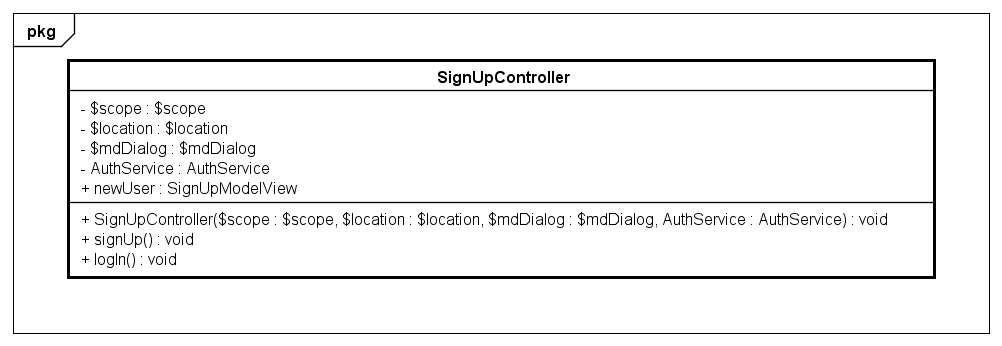
\includegraphics[scale=0.45]{UML/Classi/Front-End/QuizziPedia_Front-end_Controller_SignUpController.png}
	\caption{QuizziPedia::Front-End::Controllers::SignUpController}
\end{figure} \FloatBarrier
\begin{itemize}
	\item \textbf{Descrizione}: questa classe permette di gestire la registrazione di un utente al sistema;
	\item \textbf{Utilizzo}: fornisce le funzionalità di registrazione di un utente al sistema;
	\item \textbf{Relazione con altre classi}:
	\begin{itemize}
		\item \textit{IN} \texttt{SignUpModelView}: classe di tipo modelview la cui istanzazione è contenuta all'interno della variabile di ambiente \$scope di \textit{Angular.js\ped{G}}. All'interno di essa sono presenti le variabili e i metodi necessari per il \textit{Two-Way Data-Binding\ped{G}} tra la view \texttt{SignUpView} e il controller \texttt{SignUpController};
		\item \textit{IN} \texttt{AuthService}: questa classe permette di gestire la registrazione e l'autenticazione di un utente;
	\end{itemize}
	\item \textbf{Attributi}:
	\begin{itemize}
		\item \texttt{-} \texttt{\$scope: \$scope} \\
		Campo dati contenente un riferimento all’oggetto \$scope creato da \textit{Angular\ped{G}}. Viene utilizzato come mezzo di comunicazione tra il controller e la view. Contiene gli oggetti che definiscono il viewmodel e il model dell’applicazione;
		\item \texttt{-} \texttt{\$location: \$location} \\
		Campo dati contenente un riferimento al servizio creato da \textit{Angular\ped{G}} che permette di accedere alla barra degli indirizzi del \textit{browser\ped{G}}, i cambiamenti all’URL nella barra degli indirizzi si riflettono in questo oggetto e viceversa;
		\item \texttt{-} \texttt{\$mdDialog: \$mdDialog} \\
		Campo dati contenente un riferimento al servizio della libreria \textit{Material for Angular\ped{G}} che permette di creare delle componenti a popup;
		\item \texttt{-} \texttt{AuthService: AuthService} \\
		Campo dati contenente un riferimento al servizio che si occupa della gestione delle informazioni legate all’autenticazione. Viene utilizzato il metodo \texttt{signUp} di \$texttt{AuthService} a cui viene passato come parametro un oggetto di tipo \texttt{SignUpModelView};
		\item \texttt{+} \texttt{newUser: SignUpModelView} \\
		Oggetto di tipo \texttt{SignUpModelView}. All'interno di esso sono presenti le variabili e i metodi necessari per il \textit{Two-Way Data-Binding\ped{G}} tra la view \texttt{SignUpView} e il controller \texttt{SignUpController};
	\end{itemize}
	\item \textbf{Metodi}:
	\begin{itemize}
		\item \texttt{+} \texttt{SignUpController(\$scope: \$scope, \$location: \$location, \$mdDialog: \$mdDialog, AuthService: AuthService)} \\
		Metodo costruttore della classe: \\
		\textbf{Parametri}:
		\begin{itemize}
			\item \texttt{\$scope: \$scope} \\
			Parametro contenente un riferimento all’oggetto \$scope creato da \textit{Angular\ped{G}}. Viene utilizzato come mezzo di comunicazione tra il controller e la view. Contiene gli oggetti che definiscono il viewmodel e il model dell’applicazione;
			\item \texttt{\$location: \$location} \\
			Parametro contenente un riferimento al servizio creato da \textit{Angular\ped{G}} che permette di accedere alla barra degli indirizzi del \textit{browser\ped{G}}, i cambiamenti all’URL nella barra degli indirizzi si riflettono in questo oggetto e viceversa;
			\item \texttt{\$mdDialog: \$mdDialog} \\
			Parametro contenente un riferimento al servizio della libreria \textit{Material for Angular\ped{G}} che permette di creare delle componenti a popup;
			\item \texttt{AuthService: AuthService} \\
			Campo dati contenente un riferimento al servizio che si occupa della gestione delle informazioni legate all’autenticazione. Viene utilizzato il metodo \texttt{logIn} di \$texttt{AuthService} a cui vengono passati i parametri \texttt{username} e \texttt{password};
		\end{itemize}
		\item \texttt{+} \texttt{signUp(): void} \\
		Metodo che richiama il metodo \texttt{signUp} del service \texttt{AuthService} passandogli un oggetto di tipo \texttt{SignUpModelView}. Nel caso di buona riuscita dell'operazione viene mostrato un messaggio di successo. Con l'azione di click sul bottone presentato dal messaggio di successo è possibile effettuare il redirect alla pagina di login dell'applicazione. Nel caso in cui invece avvenga un errore, viene mostrato a video il messaggio di errore;
		\item \texttt{+} \texttt{logIn(): void} \\
		Metodo che gestisce l’evento click sul pulsante di login. Effettua il redirect alla pagina di login;
	
	\end{itemize}
\end{itemize}

\paragraph{QuizziPedia::Front-End::Controllers::HomeController}
\begin{figure} [ht]
	\centering
	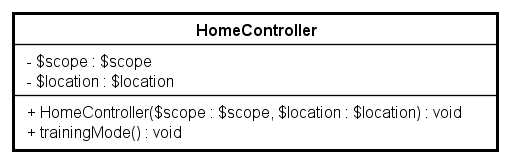
\includegraphics[scale=0.45]{UML/Classi/Front-End/QuizziPedia_Front-end_Controller_HomeController.png}
	\caption{QuizziPedia::Front-End::Controllers::HomeController}
\end{figure} \FloatBarrier
\begin{itemize}
	\item \textbf{Descrizione}: questa classe permette di gestire la home page;
	\item \textbf{Utilizzo}: fornisce tutte le informazioni da mostrare nella homepage;
	\item \textbf{Relazione con altre classi}:
	\begin{itemize}
		\item \textit{IN} \texttt{HomeModelView}: classe di tipo modelview la cui istanzazione è contenuta all'interno della variabile di ambiente \$scope di \textit{Angular.js\ped{G}}. All'interno di essa sono presenti le variabili e i metodi necessari per il \textit{Two-Way Data-Binding\ped{G}} tra la view \texttt{HomeView} e il controller \texttt{HomeController};
	\end{itemize}
	\item \textbf{Attributi}:
	\begin{itemize}
		\item \texttt{-} \texttt{\$scope: \$scope} \\
		Campo dati contenente un riferimento all’oggetto \$scope creato da \textit{Angular\ped{G}}, viene utilizzato come mezzo di comunicazione tra il controller e la view. Contiene gli oggetti che definiscono il model dell’applicazione;
		\item \texttt{-} \texttt{\$location: \$location} \\
		Campo dati contenente un riferimento al servizio creato da \textit{Angular\ped{G}} che permette di accedere alla barra degli indirizzi del \textit{browser\ped{G}}, i cambiamenti all’URL nella barra degli indirizzi si riflettono in questo oggetto e viceversa;
	\end{itemize}
	\item \textbf{Metodi}:
	\begin{itemize}
		\item \texttt{+} \texttt{HomeController(\$scope: \$scope, \$location: \$location)} \\
		Metodo costruttore della classe: \\
		\textbf{Parametri}:
		\begin{itemize}
			\item \texttt{\$scope: \$scope} \\
			Parametro contenente un riferimento all’oggetto \$scope creato da \textit{Angular\ped{G}}. Viene utilizzato come mezzo di comunicazione tra il controller e la view. Contiene gli oggetti che definiscono il viewmodel e il model dell’applicazione;
			\item \texttt{\$location: \$location} \\
			Parametro contenente un riferimento al servizio creato da \textit{Angular\ped{G}} che permette di accedere alla barra degli indirizzi del \textit{browser\ped{G}}, i cambiamenti all’URL nella barra degli indirizzi si riflettono in questo oggetto e viceversa;
		\end{itemize}
		\item \texttt{+} \texttt{trainingMode(): void} \\
		Metodo che gestisce l’evento click sul pulsante di allenamento. Effettua il redirect alla pagina di allenamento; 
	\end{itemize}
\end{itemize}

\paragraph{QuizziPedia::Front-End::Controllers::SearchController}
\begin{figure} [ht]
	\centering
	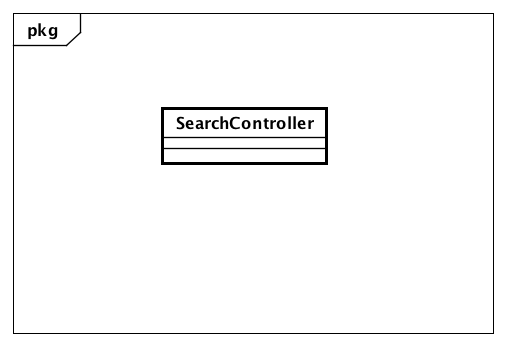
\includegraphics[scale=0.45]{UML/Classi/Front-End/QuizziPedia_Front-end_Controller_SearchController.png}
	\caption{QuizziPedia::Front-End::Controllers::SearchController}
\end{figure} \FloatBarrier
\begin{itemize}
	\item \textbf{Descrizione}: questa classe permette di gestire la ricerca di questionari e utenti all'interno dell'applicazione;
	\item \textbf{Utilizzo}: fornisce all'utente le funzionalità di ricerca per utenti e questionari;
	\item \textbf{Relazione con altre classi}:
	\begin{itemize}
		\item \textit{IN} \texttt{ResultsModelView}: classe di tipo modelview la cui istanzazione è contenuta all'interno della variabile di ambiente \$scope di \textit{Angular.js\ped{G}}. All'interno di essa sono presenti le variabili e i metodi necessari per il \textit{Two-Way Data-Binding\ped{G}} tra la view \texttt{ResultsView}, la directive \texttt{SearchDirective} e il controller \texttt{ResultsController};
		\item \textit{IN} \texttt{SearchService}: questa classe permette di eseguire una ricerca tra i questionari e gli utenti presenti ritornando un \textit{Object} contenente i risultati di tale operazione;
		\item \textit{IN} \texttt{QuizService}: questa classe permette di ottenere i dati di un quiz tramite delle parole chiave inserite dall'utente nella barra di ricerca. Permette inoltre di iscriversi ad un questionario;
	\end{itemize}
	\item \textbf{Attributi}:
	\begin{itemize}
		\item \texttt{-} \texttt{\$scope: \$scope} \\
		Campo dati contenente un riferimento all’oggetto \$scope creato da \textit{Angular\ped{G}}, viene utilizzato come mezzo di comunicazione tra il controller e la view. Contiene gli oggetti che definiscono il model dell’applicazione;
		\item \texttt{-} \texttt{\$location: \$location} \\
		Campo dati contenente un riferimento al servizio creato da \textit{Angular\ped{G}} che permette di accedere alla barra degli indirizzi del \textit{browser\ped{G}}, i cambiamenti all’URL nella barra degli indirizzi si riflettono in questo oggetto e viceversa;
		\item \texttt{-} \texttt{\$mdDialog: \$mdDialog} \\
		Campo dati contenente un riferimento al servizio della libreria \textit{Material for Angular\ped{G}} che permette di creare delle componenti a popup;
		\item \texttt{-} \texttt{SearchService: SearchService} \\
		Campo dati contenente un riferimento al servizio che si occupa della gestione delle informazioni legate alla ricerca. Viene utilizzato il metodo \texttt{search} di \$texttt{SearchService} a cui viene passato come parametro la stringa di ricerca;
		\item \texttt{-} \texttt{QuizService: QuizService} \\
		Campo dati contenente un riferimento al servizio che si occupa della gestione delle informazioni legate ai questionari. Viene utilizzato il metodo \texttt{subscribeQuestionnaire} di \$texttt{QuizService} per iscrivere un utente ad un questionario;
		\item \texttt{+} \texttt{result: SearchModelView} \\
		Oggetto di tipo \texttt{SearchModelView}. All'interno di esso sono presenti le variabili e i metodi necessari per il \textit{Two-Way Data-Binding\ped{G}} tra la view \texttt{ResultView} e il controller \texttt{SearchController};
	\end{itemize}
	\item \textbf{Metodi}:
	\begin{itemize}
		\item \texttt{+} \texttt{SearchController(\$scope: \$scope, \$location: \$location, \$mdDialog: \$mdDialog, SearchService: SearchService)} \\
		Metodo costruttore della classe. Viene eseguita la ricerca per poter poi popolare il campo dati \texttt{result}. \\
		\textbf{Parametri}:
		\begin{itemize}
			\item \texttt{\$scope: \$scope} \\
			Parametro contenente un riferimento all’oggetto \$scope creato da \textit{Angular\ped{G}}. Viene utilizzato come mezzo di comunicazione tra il controller e la view. Contiene gli oggetti che definiscono il viewmodel e il model dell’applicazione;
			\item \texttt{\$location: \$location} \\
			Parametro contenente un riferimento al servizio creato da \textit{Angular\ped{G}} che permette di accedere alla barra degli indirizzi del \textit{browser\ped{G}}, i cambiamenti all’URL nella barra degli indirizzi si riflettono in questo oggetto e viceversa;
			\item \texttt{\$mdDialog: \$mdDialog} \\
			Parametro contenente un riferimento al servizio della libreria \textit{Material for Angular\ped{G}} che permette di creare delle componenti a popup;
			\item \texttt{SearchService: SearchService} \\
			Parametro contenente un riferimento al servizio che si occupa della gestione delle informazioni legate alla ricerca. Viene utilizzato il metodo \texttt{search} di \$texttt{SearchService} a cui viene passato come parametro la stringa di ricerca;
		\end{itemize} 
		\item \texttt{-} \texttt{getSearch(stringSearch: String): SearchModelView} \\
		Metodo che esegue la ricerca utilizzando un metodo fornito dalla classe SearchService. \\
		\textbf{Parametri}:
		\begin{itemize}
			\item \texttt{stringSearch: String} \\
			Parametro contenente la stringa della quale effettuare la ricerca;
		\end{itemize} 
		\item \texttt{+} \texttt{goToUser(idUser: String): void} \\
		Metodo che gestisce l’evento click sul bottone per visualizzare il profilo dell'utente selezionato. Effettua il redirect alla pagina dell'utente.\\
		\textbf{Parametri}:
		\begin{itemize}
			\item \texttt{idUser: String} \\
			Parametro contenente l'id dell'utente di cui si vuole visualizzare il profilo;
		\end{itemize} 
		\item \texttt{+} \texttt{registrationToQuiz(idQuiz: String): void} \\
		Metodo che gestisce l’evento click sul pulsante di registrazione al questionario.\\
		\textbf{Parametri}:
		\begin{itemize}
			\item \texttt{idQuiz: String} \\
			Parametro contenente l'id del questionario di cui si vuole effettuare l'iscrizione;
		\end{itemize} 
		\item \texttt{+} \texttt{goToResultsPage(stringSearch: String): void} \\
		Metodo che gestisce l’evento click sul pulsante per effettuare una ricerca.\\
		\textbf{Parametri}:
		\begin{itemize}
			\item \texttt{stringSearch: String} \\
			Parametro contenente la stringa della quale effettuare la ricerca;
		\end{itemize} 
	\end{itemize}
\end{itemize}

\paragraph{QuizziPedia::Front-End::Controllers::ProfileManagementController}
\begin{figure} [ht]
	\centering
	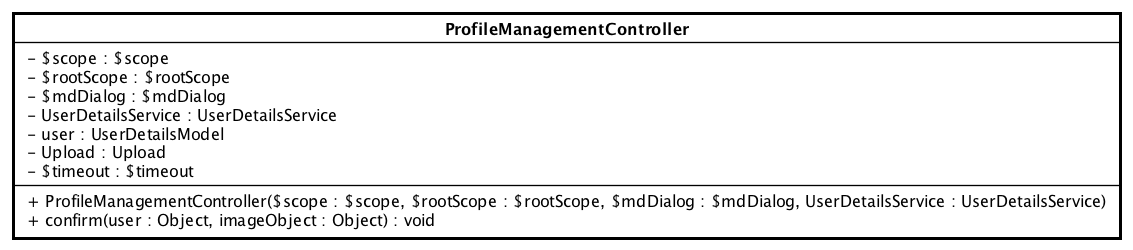
\includegraphics[scale=0.45]{UML/Classi/Front-End/QuizziPedia_Front-end_Controller_ProfileManagementController.png}
	\caption{QuizziPedia::Front-End::Controllers::ProfileManagementController}
\end{figure} \FloatBarrier
\begin{itemize}
	\item \textbf{Descrizione}: questa classe permette di gestire il profilo personale di un utente; 
	\item \textbf{Utilizzo}: fornisce le funzionalità all'utente per poter gestire i propri dati;
	\item \textbf{Relazione con altre classi}:
	\begin{itemize}
		\item \textit{IN} \texttt{ProfileManagementModelView}: classe di tipo modelview la cui istanzazione è contenuta all'interno della variabile di ambiente \$scope di \textit{Angular.js\ped{G}}. All'interno di essa sono presenti le variabili e i metodi necessari per il \textit{Two-Way Data-Binding\ped{G}} tra la view \texttt{ProfileManagementView} e il controller \texttt{ProfileManagementController};
		\item \textit{IN} \texttt{UserDetailsService}: questa classe permette di ottenere i dati personali degli utenti;
		\item \textit{IN} \texttt{UserDetailsModel}: questa classe rappresenta il tipo dell'utente autenticato della pagina; 
	\end{itemize}
	\item \textbf{Attributi}:
	\begin{itemize}
		\item \texttt{-} \texttt{\$scope: \$scope} \\
		Campo dati contenente un riferimento all’oggetto \$scope creato da \textit{Angular\ped{G}}, viene utilizzato come mezzo di comunicazione tra il controller e la view. Contiene gli oggetti che definiscono il model dell’applicazione;
		\item \texttt{-} \texttt{\$rootScope: \$rootScope} \\
		Campo dati contenente il riferimento all'oggetto globale \$rootScope creato da \textit{Angular\ped{G}}. Viene utilizzato per rendere accessibile a tutti i controller e a tutte le view l'oggetto \texttt{UserDetailsModel};
		\item \texttt{-} \texttt{\$mdDialog: \$mdDialog} \\
		Campo dati contenente un riferimento al servizio della libreria \textit{Material for Angular\ped{G}} che permette di creare delle componenti a popup;		
		\item \texttt{-} \texttt{UserDetailsService: UserDetailsService}: \\
		Campo dati contenente un riferimento al servizio che si occupa della gestione delle informazioni legate agli utenti;
		\item \texttt{+} \texttt{user: UserDetailsModel}: \\
		Oggetto di tipo \texttt{UserDetailsModel}. Viene mantenuto all'interno del \$rootScope; 
		\item \texttt{-} \texttt{Upload: Upload} \\
		Campo dati contenente un riferimento alla libreria \textit{ng-file-upload\ped{G}} necessaria per il caricamento della foto profilo dell'utente;
		\item \texttt{-} \texttt{\$timeout: \$timeout} \\
		Campo dati contenente il riferimento all'oggetto globale \$timeout creato da \textit{Angular.js\ped{G}}. 
		Il valore di ritorno di una chiamata alla funzione di \texttt{\$timeout} è una promise, la quale sarà risolta quando avverrà il ritardo e la funzione di timeout eseguita; 
	\end{itemize}
	\item \textbf{Metodi}:
	\begin{itemize}
		\item \texttt{+} \texttt{ProfileManagementController(\$scope: \$scope, \$rootScope: \$rootScope, \$mdDialog: \$mdDialog, UserDetailsService: UserDetailsService)} \\
		Metodo costruttore della classe. \\
		\textbf{Parametri}:
		\begin{itemize}
			\item \texttt{\$scope: \$scope} \\
			Parametro contenente un riferimento all’oggetto \$scope creato da \textit{Angular\ped{G}}. Viene utilizzato come mezzo di comunicazione tra il controller e la view. Contiene gli oggetti che definiscono il viewmodel e il model dell’applicazione;
			\item \texttt{\$rootScope: \$rootScope} \\
			Parametro contenente il riferimento all'oggetto globale \$rootScope creato da \textit{Angular\ped{G}}. Viene utilizzato per rendere accessibile a tutti i controller e a tutte le view l'oggetto \texttt{UserDetailsModel}. In questo caso viene utilizzato per aggiornare in \$rootScope l'oggetto che rappresenta l'utente autenticato all'interno dell'applicazione;
			\item \texttt{\$location: \$location} \\
			Parametro contenente un riferimento al servizio creato da \textit{Angular\ped{G}} che permette di accedere alla barra degli indirizzi del \textit{browser\ped{G}}, i cambiamenti all’URL nella barra degli indirizzi si riflettono in questo oggetto e viceversa;
			\item \texttt{\$mdDialog: \$mdDialog} \\
			Parametro contenente un riferimento al servizio della libreria \textit{Material for Angular\ped{G}} che permette di creare delle componenti a popup;
			\item \texttt{UserDetailsService: UserDetailsService} \\
			Parametro contenente un riferimento al servizio che si occupa della gestione delle informazioni legate all’utente;
			\item \texttt{Upload: Upload} \\
			Parametro contenente un riferimento alla libreria \textit{ng-file-upload} necessaria per il caricamento della foto profilo dell'utente;
			\item \texttt{\$timeout: \$timeout} \\
			Parametro contenente il riferimento all'oggetto globale \$timeout creato da \textit{Angular.js\ped{G}}. 
			Il valore di ritorno di una chiamata alla funzione di \texttt{\$timeout} è una promise, la quale sarà risolta quando avverrà il ritardo e la funzione di timeout eseguita; 
		\end{itemize}
		\item \texttt{+} \texttt{confirm(): void} \\
		Metodo che gestisce l’evento click sul pulsante di conferma modifica. Aggiorna, in caso di modifiche, l'oggetto locale \texttt{UserDetailsModel}. Inoltre, utilizzando il metodo dell'\texttt{UserDetailsService}, aggiorna anche nel server i dati dell'utente.
	\end{itemize}
\end{itemize}

\paragraph{QuizziPedia::Front-End::Controllers::PasswordForgotController}
\begin{figure} [ht]
	\centering
	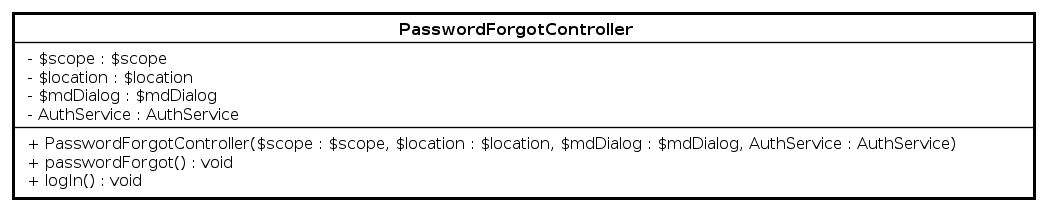
\includegraphics[scale=0.45]{UML/Classi/Front-End/QuizziPedia_Front-end_Controller_PasswordForgotController.png}
	\caption{QuizziPedia::Front-End::Controllers::PasswordForgotController}
\end{figure} \FloatBarrier
\begin{itemize}
	\item \textbf{Descrizione}: questa classe permette di gestire il ripristino della password dimenticata;
	\item \textbf{Utilizzo}: fornisce tutte le funzionalità per ripristinare la password dopo aver verificato l'identità dell'utente;
	\item \textbf{Relazione con altre classi}:
	\begin{itemize}
		\item \textit{IN} \texttt{PasswordForgotModelView}: classe di tipo modelview la cui istanzazione è contenuta all'interno della variabile di ambiente \$scope di \texttt{Angular.js}. All'interno di essa sono presenti le variabili e i metodi necessari per il \textit{Two-Way Data-Binding\ped{G}} tra la view \texttt{PasswordForgotView} e il controller \texttt{PasswordForgotController};
		\item \textit{IN} \texttt{AuthService}: questa classe permette di gestire la registrazione e l'autenticazione di un utente;
	\end{itemize}
	\item \textbf{Attributi}:
	\begin{itemize}
		\item \texttt{-} \texttt{\$scope: \$scope} \\
		Campo dati contenente un riferimento all’oggetto \$scope creato da \textit{Angular\ped{G}}, viene utilizzato come mezzo di comunicazione tra il controller e la view. Contiene gli oggetti che definiscono il model dell’applicazione;
		\item \texttt{-} \texttt{\$location: \$location} \\
		Campo dati contenente un riferimento al servizio creato da \textit{Angular\ped{G}} che permette di accedere alla barra degli indirizzi del \textit{browser\ped{G}}, i cambiamenti all’URL nella barra degli indirizzi si riflettono in questo oggetto e viceversa;
		\item \texttt{-} \texttt{\$mdDialog: \$mdDialog} \\
		Campo dati contenente un riferimento al servizio della libreria \textit{Material for Angular\ped{G}} che permette di creare delle componenti a popup;
		\item \texttt{-} \texttt{AuthService: AuthService} \\
		Campo dati contenente un riferimento al servizio che si occupa della gestione delle informazioni legate all’autenticazione. Viene utilizzato il metodo \texttt{passwordForgot} di \$texttt{AuthService} a cui viene passato il parametro \texttt{email};
	\end{itemize}
	\item \textbf{Metodi}:
	\begin{itemize}
		\item \texttt{+} \texttt{PasswordForgotController(\$scope: \$scope, \$location: \$location, \$mdDialog: \$mdDialog, AuthService: AuthService)} \\
		Metodo costruttore della classe; \\
		\textbf{Parametri}:
		\begin{itemize}
			\item \texttt{\$scope: \$scope} \\
			Parametro contenente un riferimento all’oggetto \$scope creato da \textit{Angular\ped{G}}. Viene utilizzato come mezzo di comunicazione tra il controller e la view. Contiene gli oggetti che definiscono il viewmodel e il model dell’applicazione;
			\item \texttt{\$location: \$location} \\
			Parametro contenente un riferimento al servizio creato da \textit{Angular\ped{G}} che permette di accedere alla barra degli indirizzi del \textit{browser\ped{G}}, i cambiamenti all’URL nella barra degli indirizzi si riflettono in questo oggetto e viceversa;
			\item \texttt{\$mdDialog: \$mdDialog} \\
			Parametro contenente un riferimento al servizio della libreria \textit{Material for Angular\ped{G}} che permette di creare delle componenti a popup;
			\item \texttt{AuthService: AuthService} \\
			Campo dati contenente un riferimento al servizio che si occupa della gestione delle informazioni legate all’autenticazione. Viene utilizzato il metodo \texttt{passwordForgot} di \$texttt{AuthService} a cui viene passato il parametro \texttt{email};
		\end{itemize}
		\item \texttt{+} \texttt{passwordForgot(): void} \\
		Metodo che richiama il metodo \texttt{passwordForgot} del service \texttt{AuthService} passandogli il parametro \texttt{email}. Nel caso di buona riuscita dell'operazione, viene mostrato un messaggio di successo il cui corpo contiene anche un bottone per effettuare il redirect alla pagina di login. Nel caso in cui invece avvenga un errore, viene mostrato a video il messaggio di errore;
		\item \texttt{+} \texttt{logIn(): void} \\
		Metodo che gestisce l’evento click sul pulsante di login. Effettua il redirect alla pagina di login;
	\end{itemize}
\end{itemize}

\paragraph{QuizziPedia::Front-End::Controllers::TrueFalseQuestionsController}
\begin{figure} [ht]
	\centering
	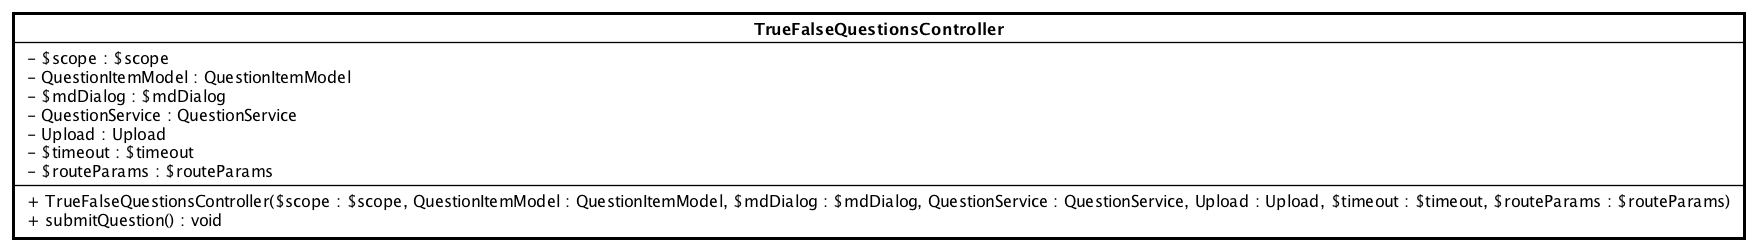
\includegraphics[scale=0.45]{UML/Classi/Front-End/QuizziPedia_Front-end_Controller_TrueFalseQuestionsController.png}
	\caption{QuizziPedia::Front-End::Controllers::TrueFalseQuestionsController}
\end{figure} \FloatBarrier
\begin{itemize}
	\item \textbf{Descrizione}: questa classe permette di gestire la creazione e la modifica di una domanda vero/falso;
	\item \textbf{Utilizzo}: fornisce le funzionalità per inserire una nuova domanda vero/falso nel database e per modificarne una esistente;
	\item \textbf{Relazione con altre classi}:
	\begin{itemize}
		\item \textit{IN} \texttt{TrueFalseQuestionsModelView}: classe di tipo modelview la cui istanzazione è contenuta all'interno della variabile di ambiente \$scope di \textit{Angular.js\ped{G}}. All'interno di essa sono presenti le variabili e i metodi necessari per il \textit{Two-Way Data-Binding\ped{G}} tra la view \texttt{TrueFalseQuestionsView} e il controller \texttt{TrueFalseQuestionsController};
		\item \textit{IN} \texttt{QuestionService}: questa classe permette di:
			\begin{itemize}
				\item Ottenere una domanda attraverso il metodo dedicato;
				\item Caricare una domanda modificata;
				\item Caricare una nuova domanda.
			\end{itemize}
		\item \textit{IN} \texttt{QuestionItemModel}: questa classe rappresenta il modello di una domanda;
	\end{itemize}
	\item \textbf{Attributi}:
	\begin{itemize}
		\item \texttt{-} \texttt{\$scope: \$scope} \\
		Campo dati contenente un riferimento all’oggetto \$scope creato da \textit{Angular\ped{G}}, viene utilizzato come mezzo di comunicazione tra il controller e la view. Contiene gli oggetti che definiscono il model dell’applicazione;
		\item \texttt{-} \texttt{QuestionItemModel: QuestionItemModel} \\
		Campo dati che si riferisce alla classe che rappresenta il modello della classe;
		\item \texttt{-} \texttt{\$mdDialog: \$mdDialog} \\
		Campo dati contenente un riferimento al servizio della libreria \textit{Material for Angular\ped{G}} che permette di creare delle componenti a popup;
		\item \texttt{-} \texttt{QuestionService: QuestionService}: \\
		Campo dati contenente un riferimento al servizio che si occupa della gestione delle informazioni legate alle domande;
		\item \texttt{-} \texttt{Upload: Upload} \\
		Campo dati contenente un riferimento alla libreria \textit{ng-file-upload\ped{G}} necessaria per il caricamento della foto profilo dell'utente;
		\item \texttt{-} \texttt{\$timeout: \$timeout} \\
		Campo dati contenente il riferimento all'oggetto globale \$timeout creato da \textit{Angular.js\ped{G}}. 
		Il valore di ritorno di una chiamata alla funzione di \texttt{\$timeout} è una promise, la quale sarà risolta quando avverrà il ritardo e la funzione di timeout eseguita; 
		\item \texttt{-} \texttt{\$routeParams: \$routeParams} \\
		Campo dati contenente il riferimento all'oggetto globale \$routeParams creato da \textit{Angular.js\ped{G}}. Tale servizio permette di recuperare il set di variabili presenti nell'url; 
	\end{itemize}
	\item \textbf{Metodi}:
	\begin{itemize}
		\item \texttt{+} \texttt{TrueFalseQuestionsController(\$scope: \$scope, QuestionItemModel: QuestionItemModel, \$mdDialog: \$mdDialog, QuestionService: QuestionService, Upload: Upload, \$timeout: \$timeout, \$routeParams: \$routeParams)} \\ 
		Metodo costruttore della classe. Se in \texttt{\$routeParams} sarà presente il codice univoco che rappresenta una domanda e di questa il creatore è l'utente autenticato, allora verrà scaricato attraverso il \texttt{QuestionService} il contenuto della domanda così da poterlo modificare. In caso contrario verrà mostrato un errore attraverso \texttt{\$mdDialog} indicando che i privilegi per tale operazione sono negati. Nel caso in cui non ci sarà tale parametro in \texttt{\$routeParams} verrà caricata la view vuota così da poter creare una nuova domanda; \\
		\textbf{Parametri}:
		\begin{itemize}
			\item \texttt{\$scope: \$scope} \\
			Parametro contenente un riferimento all’oggetto \$scope creato da \textit{Angular\ped{G}}, viene utilizzato come mezzo di comunicazione tra il controller e la view. Contiene gli oggetti che definiscono il model dell’applicazione;
			\item \texttt{QuestionItemModel: QuestionItemModel} \\ 
			Parametro che si riferisce alla classe che rappresenta il modello della classe;
			\item \texttt{\$mdDialog: \$mdDialog} \\
			Parametro contenente un riferimento al servizio della libreria \textit{Material for Angular\ped{G}} che permette di creare delle componenti a popup;
			\item \texttt{QuestionService: QuestionService}: \\
			Parametro contenente un riferimento al servizio che si occupa della gestione delle informazioni legate alle domande;
			\item \texttt{Upload: Upload} \\
			Parametro contenente un riferimento alla libreria \textit{ng-file-upload\ped{G}} necessaria per il caricamento della foto profilo dell'utente;
			\item \texttt{\$timeout: \$timeout} \\
			Parametro contenente il riferimento all'oggetto globale \$timeout creato da \textit{Angular.js\ped{G}}. 
			Il valore di ritorno di una chiamata alla funzione di \texttt{\$timeout} è una promise, la quale sarà risolta quando avverrà il ritardo e la funzione di timeout eseguita; 
			\item \texttt{\$routeParams: \$routeParams} \\
			Parametro contenente il riferimento all'oggetto globale \$routeParams creato da \textit{Angular.js\ped{G}}. Tale servizio permette di recuperare il set di variabili presenti nell'url; 
		\end{itemize}
		\item \texttt{+} \texttt{submitQuestion(): void}\\ 
		Metodo che gestisce l’evento click sul pulsante di conferma sulla domanda. Raccoglie i dati dal modelview e li manda al server attraverso \texttt{QuestionService}. Poi verrà effettuato il redirect alla pagina di gestione delle domande oppure al questionario che si stava creando; 
	\end{itemize}
\end{itemize}

\paragraph{QuizziPedia::Front-End::Controllers::MultipleQuestionsController}
\begin{figure} [ht]
	\centering
	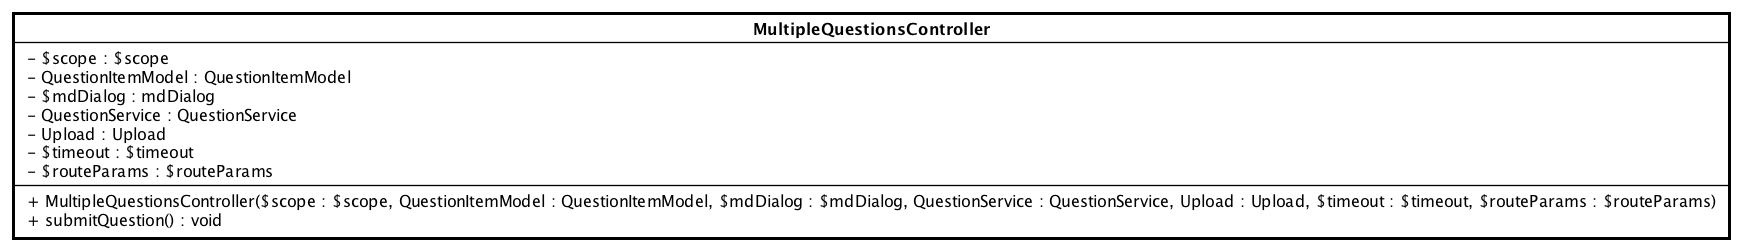
\includegraphics[scale=0.45]{UML/Classi/Front-End/QuizziPedia_Front-end_Controller_MultipleQuestionsController.png}
	\caption{QuizziPedia::Front-End::Controllers::MultipleChoiceQuestion}
\end{figure} \FloatBarrier
\begin{itemize}
	\item \textbf{Descrizione}: questa classe permette di gestire la creazione e la modifica di una domanda a risposta multipla;
	\item \textbf{Utilizzo}: fornisce le funzionalità per inserire una nuova domanda a risposta multipla nel database e per modificarne una esistente;
	\item \textbf{Relazione con altre classi}:
	\begin{itemize}
		\item \textit{IN} \texttt{MultipleQuestionsModelView}: classe di tipo modelview la cui istanzazione è contenuta all'interno della variabile di ambiente \$scope di \textit{Angular.js\ped{G}}. All'interno di essa sono presenti le variabili e i metodi necessari per il \textit{Two-Way Data-Binding\ped{G}} tra la view \texttt{MultipleQuestionsView} e il controller \texttt{MultipleQuestionsController};
		\item \textit{IN} \texttt{QuestionService}: questa classe permette di:
		\begin{itemize}
			\item Ottenere una domanda attraverso il metodo dedicato;
			\item Caricare una domanda modificata;
			\item Caricare una nuova domanda.
		\end{itemize}
		\item \textit{IN} \texttt{QuestionItemModel}: questa classe rappresenta il modello di una domanda;
	\end{itemize}
	\item \textbf{Attributi}:
	\begin{itemize}
		\item \texttt{-} \texttt{\$scope: \$scope} \\
		Campo dati contenente un riferimento all’oggetto \$scope creato da \textit{Angular\ped{G}}, viene utilizzato come mezzo di comunicazione tra il controller e la view. Contiene gli oggetti che definiscono il model dell’applicazione;
		\item \texttt{-} \texttt{QuestionItemModel: QuestionItemModel} \\
		Campo dati che si riferisce alla classe che rappresenta il modello della classe;
		\item \texttt{-} \texttt{\$mdDialog: \$mdDialog} \\
		Campo dati contenente un riferimento al servizio della libreria \textit{Material for Angular\ped{G}} che permette di creare delle componenti a popup;
		\item \texttt{-} \texttt{QuestionService: QuestionService}: \\
		Campo dati contenente un riferimento al servizio che si occupa della gestione delle informazioni legate alle domande;
		\item \texttt{-} \texttt{Upload: Upload} \\
		Campo dati contenente un riferimento alla libreria \textit{ng-file-upload\ped{G}} necessaria per il caricamento della foto profilo dell'utente;
		\item \texttt{-} \texttt{\$timeout: \$timeout} \\
		Campo dati contenente il riferimento all'oggetto globale \$timeout creato da \textit{Angular.js\ped{G}}. 
		Il valore di ritorno di una chiamata alla funzione di \texttt{\$timeout} è una promise, la quale sarà risolta quando avverrà il ritardo e la funzione di timeout eseguita; 
		\item \texttt{-} \texttt{\$routeParams: \$routeParams} \\
		Campo dati contenente il riferimento all'oggetto globale \$routeParams creato da \textit{Angular.js\ped{G}}. Tale servizio permette di recuperare il set di variabili presenti nell'url; 
	\end{itemize}
	\item \textbf{Metodi}:
	\begin{itemize}
		\item \texttt{+} \texttt{MultipleQuestionsController(\$scope: \$scope, QuestionItemModel: QuestionItemModel, \$mdDialog: \$mdDialog, QuestionService: QuestionService, Upload: Upload, \$timeout: \$timeout, \$routeParams: \$routeParams)} \\ 
		Metodo costruttore della classe. Se in \texttt{\$routeParams} sarà presente il codice univoco che rappresenta una domanda e di questa il creatore è l'utente autenticato, allora verrà scaricato attraverso il \texttt{QuestionService} il contenuto della domanda così da poterlo modificare. In caso contrario verrà mostrato un errore attraverso \texttt{\$mdDialog} indicando che i privilegi per tale operazione sono negati. Nel caso in cui non ci sarà tale parametro in \texttt{\$routeParams} verrà caricata la view vuota così da poter creare una nuova domanda; \\
		\textbf{Parametri}:
		\begin{itemize}
			\item \texttt{\$scope: \$scope} \\
			Parametro contenente un riferimento all’oggetto \$scope creato da \textit{Angular\ped{G}}, viene utilizzato come mezzo di comunicazione tra il controller e la view. Contiene gli oggetti che definiscono il model dell’applicazione;
			\item \texttt{QuestionItemModel: QuestionItemModel} \\ 
			Parametro che si riferisce alla classe che rappresenta il modello della classe;
			\item \texttt{\$mdDialog: \$mdDialog} \\
			Parametro contenente un riferimento al servizio della libreria \textit{Material for Angular\ped{G}} che permette di creare delle componenti a popup;
			\item \texttt{QuestionService: QuestionService}: \\
			Parametro contenente un riferimento al servizio che si occupa della gestione delle informazioni legate alle domande;
			\item \texttt{Upload: Upload} \\
			Parametro contenente un riferimento alla libreria \textit{ng-file-upload\ped{G}} necessaria per il caricamento della foto profilo dell'utente;
			\item \texttt{\$timeout: \$timeout} \\
			Parametro contenente il riferimento all'oggetto globale \$timeout creato da \textit{Angular.js\ped{G}}. 
			Il valore di ritorno di una chiamata alla funzione di \texttt{\$timeout} è una promise, la quale sarà risolta quando avverrà il ritardo e la funzione di timeout eseguita; 
			\item \texttt{\$routeParams: \$routeParams} \\
			Parametro contenente il riferimento all'oggetto globale \$routeParams creato da \textit{Angular.js\ped{G}}. Tale servizio permette di recuperare il set di variabili presenti nell'url; 
		\end{itemize}
		\item \texttt{+} \texttt{submitQuestion(): void}\\ 
		Metodo che gestisce l’evento click sul pulsante di conferma sulla domanda. Raccoglie i dati dal modelview e li manda al server attraverso \texttt{QuestionService}. Poi verrà effettuato il redirect alla pagina di gestione delle domande oppure al questionario che si stava creando; 
	\end{itemize}

\end{itemize}

\paragraph{QuizziPedia::Front-End::Controllers::ConnectionQuestionsController}
\begin{figure} [ht]
	\centering
	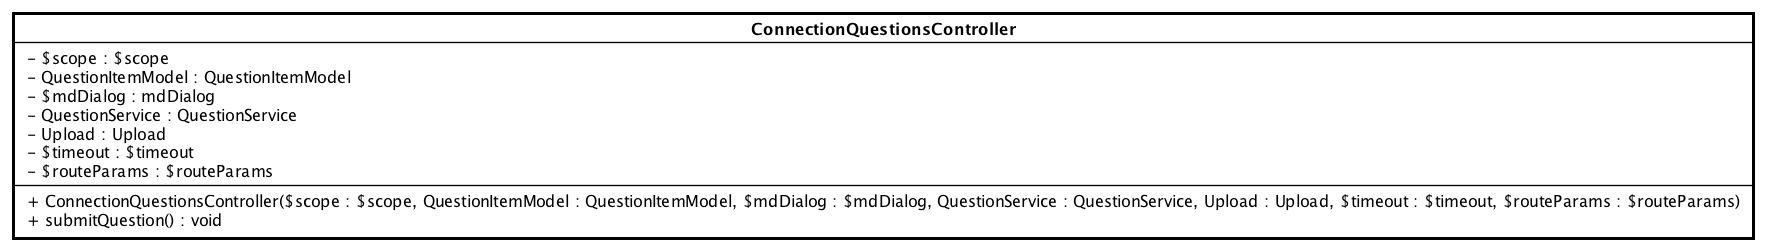
\includegraphics[scale=0.45]{UML/Classi/Front-End/QuizziPedia_Front-end_Controller_ConnectionQuestionsController.png}
	\caption{QuizziPedia::Front-End::Controllers::ConnectionQuestionsController}
\end{figure} \FloatBarrier
\begin{itemize}
	\item \textbf{Descrizione}: questa classe permette di gestire la creazione e la modifica di una domanda a collegamento;
	\item \textbf{Utilizzo}: fornisce le funzionalità per inserire una nuova domanda a collegamento nel database e per modificarne una esistente;
	\item \textbf{Relazione con altre classi}:
	\begin{itemize}
		\item \textit{IN} \texttt{ConnectionQuestionsModelView}: classe di tipo modelview la cui istanzazione è contenuta all'interno della variabile di ambiente \$scope di \textit{Angular.js\ped{G}}. All'interno di essa sono presenti le variabili e i metodi necessari per il \textit{Two-Way Data-Binding\ped{G}} tra la view \texttt{ConnectionQuestionsView} e il controller \texttt{ConnectionQuestionsController};
		\item \textit{IN} \texttt{QuestionService}: questa classe permette di:
		\begin{itemize}
			\item Ottenere una domanda attraverso il metodo dedicato;
			\item Caricare una domanda modificata;
			\item Caricare una nuova domanda.
		\end{itemize}
		\item \textit{IN} \texttt{QuestionItemModel}: questa classe rappresenta il modello di una domanda;
	\end{itemize}
	\item \textbf{Attributi}:
	\begin{itemize}
		\item \texttt{-} \texttt{\$scope: \$scope} \\
		Campo dati contenente un riferimento all’oggetto \$scope creato da \textit{Angular\ped{G}}, viene utilizzato come mezzo di comunicazione tra il controller e la view. Contiene gli oggetti che definiscono il model dell’applicazione;
		\item \texttt{-} \texttt{QuestionItemModel: QuestionItemModel} \\
		Campo dati che si riferisce alla classe che rappresenta il modello della classe;
		\item \texttt{-} \texttt{\$mdDialog: \$mdDialog} \\
		Campo dati contenente un riferimento al servizio della libreria \textit{Material for Angular\ped{G}} che permette di creare delle componenti a popup;
		\item \texttt{-} \texttt{QuestionService: QuestionService}: \\
		Campo dati contenente un riferimento al servizio che si occupa della gestione delle informazioni legate alle domande;
		\item \texttt{-} \texttt{Upload: Upload} \\
		Campo dati contenente un riferimento alla libreria \textit{ng-file-upload\ped{G}} necessaria per il caricamento della foto profilo dell'utente;
		\item \texttt{-} \texttt{\$timeout: \$timeout} \\
		Campo dati contenente il riferimento all'oggetto globale \$timeout creato da \textit{Angular.js\ped{G}}. 
		Il valore di ritorno di una chiamata alla funzione di \texttt{\$timeout} è una promise, la quale sarà risolta quando avverrà il ritardo e la funzione di timeout eseguita; 
		\item \texttt{\$routeParams: \$routeParams} \\
		Campo dati contenente il riferimento all'oggetto globale \$routeParams creato da \textit{Angular.js\ped{G}}. Tale servizio permette di recuperare il set di variabili presenti nell'url; 
	\end{itemize}
	\item \textbf{Metodi}:
	\begin{itemize}
		\item \texttt{+} \texttt{ConnectionQuestionsController(\$scope: \$scope, QuestionItemModel: QuestionItemModel, \$mdDialog: \$mdDialog, QuestionService: QuestionService, Upload: Upload, \$timeout: \$timeout, \$routeParams: \$routeParams)} \\ 
		Metodo costruttore della classe. Se in \texttt{\$routeParams} sarà presente il codice univoco che rappresenta una domanda e di questa il creatore è l'utente autenticato, allora verrà scaricato attraverso il \texttt{QuestionService} il contenuto della domanda così da poterlo modificare. In caso contrario verrà mostrato un errore attraverso \texttt{\$mdDialog} indicando che i privilegi per tale operazione sono negati. Nel caso in cui non ci sarà tale parametro in \texttt{\$routeParams} verrà caricata la view vuota così da poter creare una nuova domanda; \\
		\textbf{Parametri}:
		\begin{itemize}
			\item \texttt{\$scope: \$scope} \\
			Parametro contenente un riferimento all’oggetto \$scope creato da \textit{Angular\ped{G}}, viene utilizzato come mezzo di comunicazione tra il controller e la view. Contiene gli oggetti che definiscono il model dell’applicazione;
			\item \texttt{QuestionItemModel: QuestionItemModel} \\ 
			Parametro che si riferisce alla classe che rappresenta il modello della classe;
			\item \texttt{\$mdDialog: \$mdDialog} \\
			Parametro contenente un riferimento al servizio della libreria \textit{Material for Angular\ped{G}} che permette di creare delle componenti a popup;
			\item \texttt{QuestionService: QuestionService}: \\
			Parametro contenente un riferimento al servizio che si occupa della gestione delle informazioni legate alle domande;
			\item \texttt{Upload: Upload} \\
			Parametro contenente un riferimento alla libreria \textit{ng-file-upload\ped{G}} necessaria per il caricamento della foto profilo dell'utente;
			\item \texttt{\$timeout: \$timeout} \\
			Parametro contenente il riferimento all'oggetto globale \$timeout creato da \textit{Angular.js\ped{G}}. 
			Il valore di ritorno di una chiamata alla funzione di \texttt{\$timeout} è una promise, la quale sarà risolta quando avverrà il ritardo e la funzione di timeout eseguita; 
			\item \texttt{\$routeParams: \$routeParams} \\
			Parametro contenente il riferimento all'oggetto globale \$routeParams creato da \textit{Angular.js\ped{G}}. Tale servizio permette di recuperare il set di variabili presenti nell'url; 
		\end{itemize}
		\item \texttt{+} \texttt{submitQuestion(): void}\\ 
		Metodo che gestisce l’evento click sul pulsante di conferma sulla domanda. Raccoglie i dati dal modelview e li manda al server attraverso \texttt{QuestionService}. Poi verrà effettuato il redirect alla pagina di gestione delle domande oppure al questionario che si stava creando; 
	\end{itemize}
\end{itemize}

\paragraph{QuizziPedia::Front-End::Controllers::ImagesSortingQuestionsController}
\begin{figure} [ht]
	\centering
	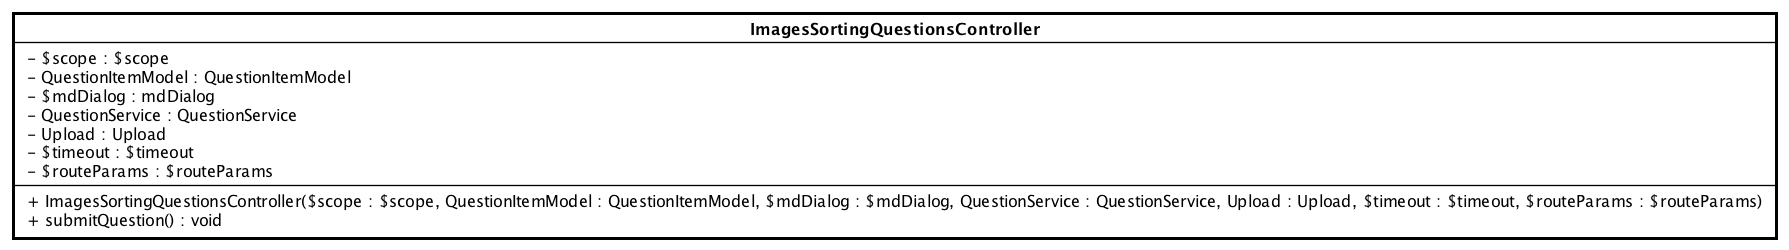
\includegraphics[scale=0.45]{UML/Classi/Front-End/QuizziPedia_Front-end_Controller_ImagesSortingQuestionsController.png}
	\caption{QuizziPedia::Front-End::Controllers::ImagesSortingQuestionsController}
\end{figure} \FloatBarrier
\begin{itemize}
	\item \textbf{Descrizione}: questa classe permette di gestire la creazione e la modifica di una domanda a ordinamento immagini;
	\item \textbf{Utilizzo}: fornisce le funzionalità per inserire una nuova domanda a ordinamento immagini nel database e per modificarne una esistente;
	\item \textbf{Relazione con altre classi}:
	\begin{itemize}
		\item \textit{IN} \texttt{ImageSortingQuestionsModelView}: classe di tipo modelview la cui istanzazione è contenuta all'interno della variabile di ambiente \$scope di \textit{Angular.js\ped{G}}. All'interno di essa sono presenti le variabili e i metodi necessari per il \textit{Two-Way Data-Binding\ped{G}} tra la view \texttt{ImagesSortingQuestionsView} e il controller \texttt{ImagesSortingQuestionsController};
		\item \textit{IN} \texttt{QuestionService}: questa classe permette di:
		\begin{itemize}
			\item Ottenere una domanda attraverso il metodo dedicato;
			\item Caricare una domanda modificata;
			\item Caricare una nuova domanda.
		\end{itemize}
		\item \textit{IN} \texttt{QuestionItemModel}: questa classe rappresenta il modello di una domanda;
	\end{itemize}
	\item \textbf{Attributi}:
	\begin{itemize}
		\item \texttt{-} \texttt{\$scope: \$scope} \\
		Campo dati contenente un riferimento all’oggetto \$scope creato da \textit{Angular\ped{G}}, viene utilizzato come mezzo di comunicazione tra il controller e la view. Contiene gli oggetti che definiscono il model dell’applicazione;
		\item \texttt{-} \texttt{QuestionItemModel: QuestionItemModel} \\
		Campo dati che si riferisce alla classe che rappresenta il modello della classe;
		\item \texttt{-} \texttt{\$mdDialog: \$mdDialog} \\
		Campo dati contenente un riferimento al servizio della libreria \textit{Material for Angular\ped{G}} che permette di creare delle componenti a popup;
		\item \texttt{-} \texttt{QuestionService: QuestionService}: \\
		Campo dati contenente un riferimento al servizio che si occupa della gestione delle informazioni legate alle domande;
		\item \texttt{-} \texttt{Upload: Upload} \\
		Campo dati contenente un riferimento alla libreria \textit{ng-file-upload\ped{G}} necessaria per il caricamento della foto profilo dell'utente;
		\item \texttt{-} \texttt{\$timeout: \$timeout} \\
		Campo dati contenente il riferimento all'oggetto globale \$timeout creato da \textit{Angular.js\ped{G}}. 
		Il valore di ritorno di una chiamata alla funzione di \texttt{\$timeout} è una promise, la quale sarà risolta quando avverrà il ritardo e la funzione di timeout eseguita; 
		\item \texttt{\$routeParams: \$routeParams} \\
		Campo dati contenente il riferimento all'oggetto globale \$routeParams creato da \textit{Angular.js\ped{G}}. Tale servizio permette di recuperare il set di variabili presenti nell'url; 
	\end{itemize}
	\item \textbf{Metodi}:
	\begin{itemize}
		\item \texttt{+} \texttt{ImageSortingQuestionsController(\$scope: \$scope, QuestionItemModel: QuestionItemModel, \$mdDialog: \$mdDialog, QuestionService: QuestionService, Upload: Upload, \$timeout: \$timeout, \$routeParams: \$routeParams)} \\ 
		Metodo costruttore della classe. Se in \texttt{\$routeParams} sarà presente il codice univoco che rappresenta una domanda e di questa il creatore è l'utente autenticato, allora verrà scaricato attraverso il \texttt{QuestionService} il contenuto della domanda così da poterlo modificare. In caso contrario verrà mostrato un errore attraverso \texttt{\$mdDialog} indicando che i privilegi per tale operazione sono negati. Nel caso in cui non ci sarà tale parametro in \texttt{\$routeParams} verrà caricata la view vuota così da poter creare una nuova domanda; \\
		\textbf{Parametri}:
		\begin{itemize}
			\item \texttt{\$scope: \$scope} \\
			Parametro contenente un riferimento all’oggetto \$scope creato da \textit{Angular\ped{G}}, viene utilizzato come mezzo di comunicazione tra il controller e la view. Contiene gli oggetti che definiscono il model dell’applicazione;
			\item \texttt{QuestionItemModel: QuestionItemModel} \\ 
			Parametro che si riferisce alla classe che rappresenta il modello della classe;
			\item \texttt{\$mdDialog: \$mdDialog} \\
			Parametro contenente un riferimento al servizio della libreria \textit{Material for Angular\ped{G}} che permette di creare delle componenti a popup;
			\item \texttt{QuestionService: QuestionService}: \\
			Parametro contenente un riferimento al servizio che si occupa della gestione delle informazioni legate alle domande;
			\item \texttt{Upload: Upload} \\
			Parametro contenente un riferimento alla libreria \textit{ng-file-upload\ped{G}} necessaria per il caricamento della foto profilo dell'utente;
			\item \texttt{\$timeout: \$timeout} \\
			Parametro contenente il riferimento all'oggetto globale \$timeout creato da \textit{Angular.js\ped{G}}. 
			Il valore di ritorno di una chiamata alla funzione di \texttt{\$timeout} è una promise, la quale sarà risolta quando avverrà il ritardo e la funzione di timeout eseguita; 
			\item \texttt{\$routeParams: \$routeParams} \\
			Parametro contenente il riferimento all'oggetto globale \$routeParams creato da \textit{Angular.js\ped{G}}. Tale servizio permette di recuperare il set di variabili presenti nell'url; 
		\end{itemize}
		\item \texttt{+} \texttt{submitQuestion(): void}\\ 
		Metodo che gestisce l’evento click sul pulsante di conferma sulla domanda. Raccoglie i dati dal modelview e li manda al server attraverso \texttt{QuestionService}. Poi verrà effettuato il redirect alla pagina di gestione delle domande oppure al questionario che si stava creando; 
	\end{itemize}
\end{itemize}

\paragraph{QuizziPedia::Front-End::Controllers::StringsSortingQuestionsController}
\begin{figure} [ht]
	\centering
	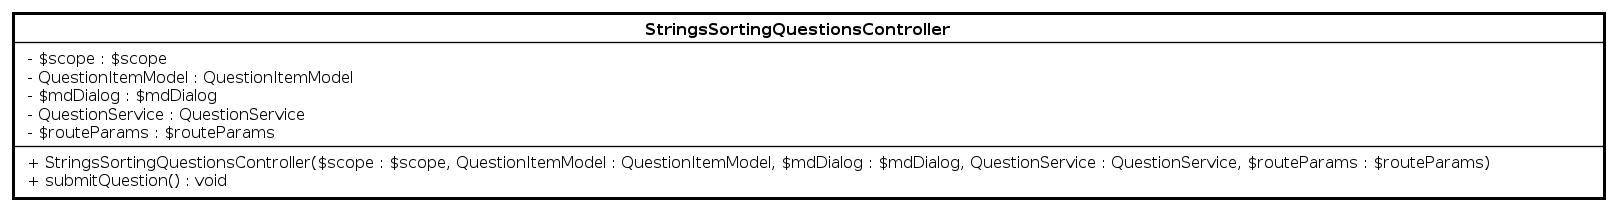
\includegraphics[scale=0.45]{UML/Classi/Front-End/QuizziPedia_Front-end_Controller_StringSortingQuestionsController.png}
	\caption{QuizziPedia::Front-End::Controllers::StringsSortingQuestionsController}
\end{figure} \FloatBarrier
\begin{itemize}
	\item \textbf{Descrizione}: questa classe permette di gestire la creazione e la modifica di una domanda a ordinamento di stringhe;
	\item \textbf{Utilizzo}: fornisce le funzionalità per inserire una nuova domanda a ordinamento di stringhe nel database e per modificarne una esistente;
	\item \textbf{Relazione con altre classi}:
	\begin{itemize}
		\item \textit{IN} \texttt{StringsSortingQuestionsModelView}: classe di tipo modelview la cui istanzazione è contenuta all'interno della variabile di ambiente \$scope di \textit{Angular.js\ped{G}}. All'interno di essa sono presenti le variabili e i metodi necessari per il \textit{Two-Way Data-Binding\ped{G}} tra la view \texttt{StringsSortingQuestionsView} e il controller \texttt{StringsSortingQuestionsController};
		\item \textit{IN} \texttt{QuestionService}: questa classe permette di:
		\begin{itemize}
			\item Ottenere una domanda attraverso il metodo dedicato;
			\item Caricare una domanda modificata;
			\item Caricare una nuova domanda.
		\end{itemize}
		\item \textit{IN} \texttt{QuestionItemModel}: questa classe rappresenta il modello di una domanda;
	\end{itemize}
	\item \textbf{Attributi}:
	\begin{itemize}
		\item \texttt{-} \texttt{\$scope: \$scope} \\
		Campo dati contenente un riferimento all’oggetto \$scope creato da \textit{Angular\ped{G}}, viene utilizzato come mezzo di comunicazione tra il controller e la view. Contiene gli oggetti che definiscono il model dell’applicazione;
		\item \texttt{-} \texttt{QuestionItemModel: QuestionItemModel} \\
		Campo dati che si riferisce alla classe che rappresenta il modello della classe;
		\item \texttt{-} \texttt{\$mdDialog: \$mdDialog} \\
		Campo dati contenente un riferimento al servizio della libreria \textit{Material for Angular\ped{G}} che permette di creare delle componenti a popup;
		\item \texttt{-} \texttt{QuestionService: QuestionService}: \\
		Campo dati contenente un riferimento al servizio che si occupa della gestione delle informazioni legate alle domande;
		\item \texttt{\$routeParams: \$routeParams} \\
		Campo dati contenente il riferimento all'oggetto globale \$routeParams creato da \textit{Angular.js\ped{G}}. Tale servizio permette di recuperare il set di variabili presenti nell'url; 
	\end{itemize}
	\item \textbf{Metodi}:
	\begin{itemize}
		\item \texttt{+} \texttt{StringsSortingQuestionsController(\$scope: \$scope, QuestionItemModel: QuestionItemModel, \$mdDialog: \$mdDialog, QuestionService: QuestionService, \$routeParams: \$routeParams)} \\ 
		Metodo costruttore della classe. Se in \texttt{\$routeParams} sarà presente il codice univoco che rappresenta una domanda e di questa il creatore è l'utente autenticato, allora verrà scaricato attraverso il \texttt{QuestionService} il contenuto della domanda così da poterlo modificare. In caso contrario verrà mostrato un errore attraverso \texttt{\$mdDialog} indicando che i privilegi per tale operazione sono negati. Nel caso in cui non ci sarà tale parametro in \texttt{\$routeParams} verrà caricata la view vuota così da poter creare una nuova domanda; \\
		\textbf{Parametri}:
		\begin{itemize}
			\item \texttt{\$scope: \$scope} \\
			Parametro contenente un riferimento all’oggetto \$scope creato da \textit{Angular\ped{G}}, viene utilizzato come mezzo di comunicazione tra il controller e la view. Contiene gli oggetti che definiscono il model dell’applicazione;
			\item \texttt{QuestionItemModel: QuestionItemModel} \\ 
			Parametro che si riferisce alla classe che rappresenta il modello della classe;
			\item \texttt{\$mdDialog: \$mdDialog} \\
			Parametro contenente un riferimento al servizio della libreria \textit{Material for Angular\ped{G}} che permette di creare delle componenti a popup;
			\item \texttt{QuestionService: QuestionService}: \\
			Parametro contenente un riferimento al servizio che si occupa della gestione delle informazioni legate alle domande;
			\item \texttt{\$routeParams: \$routeParams} \\
			Parametro contenente il riferimento all'oggetto globale \$routeParams creato da \textit{Angular.js\ped{G}}. Tale servizio permette di recuperare il set di variabili presenti nell'url; 
		\end{itemize}
		\item \texttt{+} \texttt{submitQuestion(): void}\\ 
		Metodo che gestisce l’evento click sul pulsante di conferma sulla domanda. Raccoglie i dati dal modelview e li manda al server attraverso \texttt{QuestionService}. Poi verrà effettuato il redirect alla pagina di gestione delle domande oppure al questionario che si stava creando; 
	\end{itemize}
\end{itemize}

\paragraph{QuizziPedia::Front-End::Controllers::FillingQuestionsController}
\begin{figure} [ht]
	\centering
	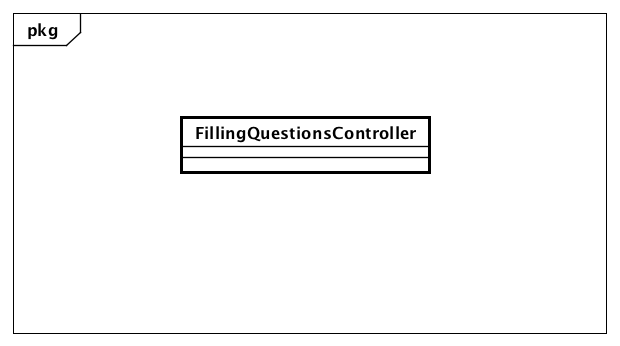
\includegraphics[scale=0.45]{UML/Classi/Front-End/QuizziPedia_Front-end_Controller_FillingQuestionsController.png}
	\caption{QuizziPedia::Front-End::Controllers::FillingQuestionsController}
\end{figure} \FloatBarrier
\begin{itemize}
	\item \textbf{Descrizione}: questa classe permette di gestire la creazione e la modifica di una domanda a riempimento di spazi;
	\item \textbf{Utilizzo}: fornisce le funzionalità per inserire una nuova domanda ariempimento di spazi nel database e per modificarne una esistente;
	\item \textbf{Relazione con altre classi}:
	\begin{itemize}
		\item \textit{IN} \texttt{FillingQuestionsModelView}: classe di tipo modelview la cui istanzazione è contenuta all'interno della variabile di ambiente \$scope di \textit{Angular.js\ped{G}}. All'interno di essa sono presenti le variabili e i metodi necessari per il \textit{Two-Way Data-Binding\ped{G}} tra la view \texttt{FillingQuestionsView} e il controller \texttt{FillingQuestionsController};
		\item \textit{IN} \texttt{QuestionService}: questa classe permette di:
		\begin{itemize}
			\item Ottenere una domanda attraverso il metodo dedicato;
			\item Caricare una domanda modificata;
			\item Caricare una nuova domanda.
		\end{itemize}
		\item \textit{IN} \texttt{QuestionItemModel}: questa classe rappresenta il modello di una domanda;
	\end{itemize}
	\item \textbf{Attributi}:
	\begin{itemize}
		\item \texttt{-} \texttt{\$scope: \$scope} \\
		Campo dati contenente un riferimento all’oggetto \$scope creato da \textit{Angular\ped{G}}, viene utilizzato come mezzo di comunicazione tra il controller e la view. Contiene gli oggetti che definiscono il model dell’applicazione;
		\item \texttt{-} \texttt{QuestionItemModel: QuestionItemModel} \\
		Campo dati che si riferisce alla classe che rappresenta il modello della classe;
		\item \texttt{-} \texttt{\$mdDialog: \$mdDialog} \\
		Campo dati contenente un riferimento al servizio della libreria \textit{Material for Angular\ped{G}} che permette di creare delle componenti a popup;
		\item \texttt{-} \texttt{QuestionService: QuestionService}: ;
		\item \texttt{\$routeParams: \$routeParams} \\
		Campo dati contenente il riferimento all'oggetto globale \$routeParams creato da \textit{Angular.js\ped{G}}. Tale servizio permette di recuperare il set di variabili presenti nell'url; 
	\end{itemize}
	\item \textbf{Metodi}:
	\begin{itemize}
		\item \texttt{+} \texttt{FillingQuestionsController(\$scope: \$scope, QuestionItemModel: QuestionItemModel, \$mdDialog: \$mdDialog, QuestionService: QuestionService)} \\ 
		Metodo costruttore della classe. Se in \texttt{\$routeParams} sarà presente il codice univoco che rappresenta una domanda e di questa il creatore è l'utente autenticato, allora verrà scaricato attraverso il \texttt{QuestionService} il contenuto della domanda così da poterlo modificare. In caso contrario verrà mostrato un errore attraverso \texttt{\$mdDialog} indicando che i privilegi per tale operazione sono negati. Nel caso in cui non ci sarà tale parametro in \texttt{\$routeParams} verrà caricata la view vuota così da poter creare una nuova domanda; \\
		\textbf{Parametri}:
		\begin{itemize}
			\item \texttt{\$scope: \$scope} \\
			Parametro contenente un riferimento all’oggetto \$scope creato da \textit{Angular\ped{G}}, viene utilizzato come mezzo di comunicazione tra il controller e la view. Contiene gli oggetti che definiscono il model dell’applicazione;
			\item \texttt{QuestionItemModel: QuestionItemModel} \\ 
			Parametro che si riferisce alla classe che rappresenta il modello della classe;
			\item \texttt{\$mdDialog: \$mdDialog} \\
			Parametro contenente un riferimento al servizio della libreria \textit{Material for Angular\ped{G}} che permette di creare delle componenti a popup;
			\item \texttt{QuestionService: QuestionService}: \\
			Parametro contenente un riferimento al servizio che si occupa della gestione delle informazioni legate alle domande;
			\item \texttt{Upload: Upload} \\
			Parametro contenente un riferimento alla libreria \textit{ng-file-upload\ped{G}} necessaria per il caricamento della foto profilo dell'utente;
			\item \texttt{\$timeout: \$timeout} \\
			Parametro contenente il riferimento all'oggetto globale \$timeout creato da \textit{Angular.js\ped{G}}. 
			Il valore di ritorno di una chiamata alla funzione di \texttt{\$timeout} è una promise, la quale sarà risolta quando avverrà il ritardo e la funzione di timeout eseguita; 
			\item \texttt{\$routeParams: \$routeParams} \\
			Parametro contenente il riferimento all'oggetto globale \$routeParams creato da \textit{Angular.js\ped{G}}. Tale servizio permette di recuperare il set di variabili presenti nell'url; 
		\end{itemize}
		\item \texttt{+} \texttt{submitQuestion(): void}\\ 
		Metodo che gestisce l’evento click sul pulsante di conferma sulla domanda. Raccoglie i dati dal modelview e li manda al server attraverso \texttt{QuestionService}. Poi verrà effettuato il redirect alla pagina di gestione delle domande oppure al questionario che si stava creando; 
		\item \texttt{+} \texttt{choseThatWord(word:String, number: Integer): void}\\
		Metodo che gestisce l’evento click su una parola del testo. Una volta selezionata essa verrà inserita nell'array che conterrà le parole che dovranno essere nascoste quando l'esercizio sarà proposto; \\
		\textbf{Parametri}:
		\begin{itemize}
			\item \texttt{word:String} \\
			Parametro contenente la parola scelta da nascondere;
			\item \texttt{number: Integer} \\ 
			Parametro che si riferisce al numero della parola scelta da nascondere;
		\end{itemize}
	\end{itemize}
\end{itemize}

\paragraph{QuizziPedia::Front-End::Controllers::ClickableAreaQuestionsController}
\begin{figure} [ht]
	\centering
	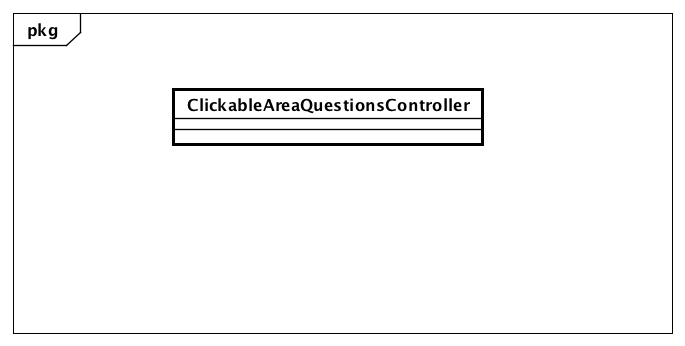
\includegraphics[scale=0.45]{UML/Classi/Front-End/QuizziPedia_Front-end_Controller_ClickableAreaQuestionsController.png}
	\caption{QuizziPedia::Front-End::Controllers::ClickableAreaQuestionsController}
\end{figure} \FloatBarrier
\begin{itemize}
	\item \textbf{Descrizione}: questa classe permette di gestire la creazione e la modifica di una domanda ad area cliccabile;
	\item \textbf{Utilizzo}: fornisce le funzionalità per inserire una nuova domanda ad area cliccabile nel database e per modificarne una esistente;
	\begin{itemize}
		\item \textit{IN} \texttt{ClickableAreaQuestionsModelView}: classe di tipo modelview la cui istanzazione è contenuta all'interno della variabile di ambiente \$scope di \textit{Angular.js\ped{G}}. All'interno di essa sono presenti le variabili e i metodi necessari per il \textit{Two-Way Data-Binding\ped{G}} tra la view \texttt{ClickableAreaQuestionsView} e il controller \texttt{ClickableAreaQuestionsController};
		\item \textit{IN} \texttt{QuestionService}: questa classe permette di:
		\begin{itemize}
			\item Ottenere una domanda attraverso il metodo dedicato;
			\item Caricare una domanda modificata;
			\item Caricare una nuova domanda.
		\end{itemize}
		\item \textit{IN} \texttt{QuestionItemModel}: questa classe rappresenta il modello di una domanda;
	\end{itemize}
	\item \textbf{Attributi}:
	\begin{itemize}
		\item \texttt{-} \texttt{\$scope: \$scope} \\
		Campo dati contenente un riferimento all’oggetto \$scope creato da \textit{Angular\ped{G}}, viene utilizzato come mezzo di comunicazione tra il controller e la view. Contiene gli oggetti che definiscono il model dell’applicazione;
		\item \texttt{-} \texttt{QuestionItemModel: QuestionItemModel} \\
		Campo dati che si riferisce alla classe che rappresenta il modello della classe;
		\item \texttt{-} \texttt{\$mdDialog: \$mdDialog} \\
		Campo dati contenente un riferimento al servizio della libreria \textit{Material for Angular\ped{G}} che permette di creare delle componenti a popup;
		\item \texttt{-} \texttt{QuestionService: QuestionService}: \\
		Campo dati contenente un riferimento al servizio che si occupa della gestione delle informazioni legate alle domande;
		\item \texttt{-} \texttt{Upload: Upload} \\
		Campo dati contenente un riferimento alla libreria \textit{ng-file-upload\ped{G}} necessaria per il caricamento della foto profilo dell'utente;
		\item \texttt{-} \texttt{\$timeout: \$timeout} \\
		Campo dati contenente il riferimento all'oggetto globale \$timeout creato da \textit{Angular.js\ped{G}}. 
		Il valore di ritorno di una chiamata alla funzione di \texttt{\$timeout} è una promise, la quale sarà risolta quando avverrà il ritardo e la funzione di timeout eseguita; 
		\item \texttt{\$routeParams: \$routeParams} \\
		Campo dati contenente il riferimento all'oggetto globale \$routeParams creato da \textit{Angular.js\ped{G}}. Tale servizio permette di recuperare il set di variabili presenti nell'url; 
	\end{itemize}
	\item \textbf{Metodi}:
	\begin{itemize}
		\item \texttt{+} \texttt{ClickableAreaQuestionsController(\$scope: \$scope, QuestionItemModel: QuestionItemModel, \$mdDialog: \$mdDialog, QuestionService: QuestionService, Upload: Upload, \$timeout: \$timeout, \$routeParams: \$routeParams)} \\ 
		Metodo costruttore della classe. Se in \texttt{\$routeParams} sarà presente il codice univoco che rappresenta una domanda e di questa il creatore è l'utente autenticato, allora verrà scaricato attraverso il \texttt{QuestionService} il contenuto della domanda così da poterlo modificare. In caso contrario verrà mostrato un errore attraverso \texttt{\$mdDialog} indicando che i privilegi per tale operazione sono negati. Nel caso in cui non ci sarà tale parametro in \texttt{\$routeParams} verrà caricata la view vuota così da poter creare una nuova domanda; \\
		\textbf{Parametri}:
		\begin{itemize}
			\item \texttt{\$scope: \$scope} \\
			Parametro contenente un riferimento all’oggetto \$scope creato da \textit{Angular\ped{G}}, viene utilizzato come mezzo di comunicazione tra il controller e la view. Contiene gli oggetti che definiscono il model dell’applicazione;
			\item \texttt{QuestionItemModel: QuestionItemModel} \\ 
			Parametro che si riferisce alla classe che rappresenta il modello della classe;
			\item \texttt{\$mdDialog: \$mdDialog} \\
			Parametro contenente un riferimento al servizio della libreria \textit{Material for Angular\ped{G}} che permette di creare delle componenti a popup;
			\item \texttt{QuestionService: QuestionService}: \\
			Parametro contenente un riferimento al servizio che si occupa della gestione delle informazioni legate alle domande;
			\item \texttt{Upload: Upload} \\
			Parametro contenente un riferimento alla libreria \textit{ng-file-upload\ped{G}} necessaria per il caricamento della foto profilo dell'utente;
			\item \texttt{\$timeout: \$timeout} \\
			Parametro contenente il riferimento all'oggetto globale \$timeout creato da \textit{Angular.js\ped{G}}. 
			Il valore di ritorno di una chiamata alla funzione di \texttt{\$timeout} è una promise, la quale sarà risolta quando avverrà il ritardo e la funzione di timeout eseguita; 
			\item \texttt{\$routeParams: \$routeParams} \\
			Parametro contenente il riferimento all'oggetto globale \$routeParams creato da \textit{Angular.js\ped{G}}. Tale servizio permette di recuperare il set di variabili presenti nell'url; 
		\end{itemize}
		\item \texttt{+} \texttt{submitQuestion(): void}\\ 
		Metodo che gestisce l’evento click sul pulsante di conferma sulla domanda. Raccoglie i dati dal modelview e li manda al server attraverso \texttt{QuestionService}. Poi verrà effettuato il redirect alla pagina di gestione delle domande oppure al questionario che si stava creando; 
		\item \texttt{+} \texttt{choseThatPoint(x:Integer, y: Integer): void}\\
		Metodo che gestisce l’evento click su un punto dell'immagine. Una volta selezionato esso verrà inserito nell'array di punti; \\
		\textbf{Parametri}:
		\begin{itemize}
			\item \texttt{x: Integer} \\
			Parametro contenente la coordinata x del punto;
			\item \texttt{y: Integer} \\ 
			Parametro contenente la coordinata y del punto;
		\end{itemize}
	\end{itemize}
\end{itemize}

\paragraph{QuizziPedia::Front-End::Controllers::EditorQMLController}
\begin{figure} [ht]
	\centering
	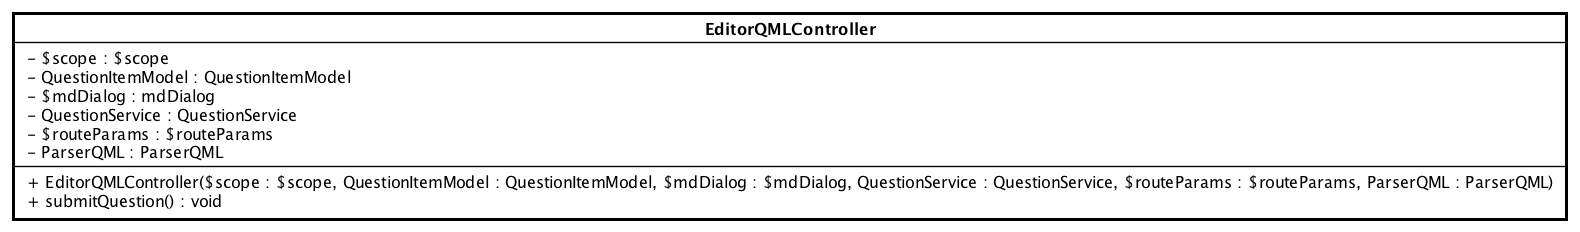
\includegraphics[scale=0.45]{UML/Classi/Front-End/QuizziPedia_Front-end_Controller_EditorQMLController.png}
	\caption{QuizziPedia::Front-End::Controllers::EditorQMLController}
\end{figure} \FloatBarrier
\begin{itemize}
	\item \textbf{Descrizione}: questa classe permette di gestire la creazione e la modifica di domande create tramite editor QML;
	\item \textbf{Utilizzo}: fornisce le funzionalità per creare e modificare una domanda tramite editor QML;
	\item \textbf{Relazione con altre classi}:
	\begin{itemize}
		\item \textit{IN} \texttt{EditorQMLModelView}: classe di tipo modelview la cui istanzazione è contenuta all'interno della variabile di ambiente \$scope di \textit{Angular.js\ped{G}}. All'interno di essa sono presenti le variabili e i metodi necessari per il \textit{Two-Way Data-Binding\ped{G}} tra la view \texttt{EditorQMLView} e il controller \texttt{EditorQMLController};
		\item \textit{IN} \texttt{QuestionService}: questa classe permette di:
		\begin{itemize}
			\item Ottenere una domanda attraverso il metodo dedicato;
			\item Caricare una domanda modificata;
			\item Caricare una nuova domanda.
		\end{itemize}
		\item \textit{IN} \texttt{ParserQML}: questa classe rappresenta il parser QML. Essa fa diventale un oggetto di tipo \texttt{QuestionItemModel} in linguaggio QML e viceversa;
		\item \textit{IN} \texttt{QuestionItemModel}: questa classe rappresenta il modello di una domanda;
	\end{itemize}
	\item \textbf{Attributi}:
	\begin{itemize}
		\item \texttt{-} \texttt{\$scope: \$scope} \\
		Campo dati contenente un riferimento all’oggetto \$scope creato da \textit{Angular\ped{G}}, viene utilizzato come mezzo di comunicazione tra il controller e la view. Contiene gli oggetti che definiscono il model dell’applicazione;
		\item \texttt{-} \texttt{QuestionItemModel: QuestionItemModel} \\
		Campo dati che si riferisce alla classe che rappresenta il modello della classe;
		\item \texttt{-} \texttt{\$mdDialog: \$mdDialog} \\
		Campo dati contenente un riferimento al servizio della libreria \textit{Material for Angular\ped{G}} che permette di creare delle componenti a popup;
		\item \texttt{-} \texttt{QuestionService: QuestionService}: \\
		Campo dati contenente un riferimento al servizio che si occupa della gestione delle informazioni legate alle domande; 
		\item \texttt{-} \texttt{\$routeParams: \$routeParams} \\
		Campo dati contenente il riferimento all'oggetto globale \$routeParams creato da \textit{Angular.js\ped{G}}. Tale servizio permette di recuperare il set di variabili presenti nell'url; 
		\item \texttt{-} \texttt{ParserQML: ParserQML} \\
		Campo dati che si riferisce alla classe che rappresenta il parser QML. Essa fa diventale un oggetto di tipo \texttt{QuestionItemModel} in linguaggio QML e viceversa;
	\end{itemize}
	\item \textbf{Metodi}:
	\begin{itemize}
		\item \texttt{+} \texttt{EditorQMLController(\$scope: \$scope, QuestionItemModel: QuestionItemModel, \$mdDialog: \$mdDialog, QuestionService: QuestionService, \$routeParams: \$routeParams, ParserQML: ParserQML)} \\ 
		Metodo costruttore della classe. Se in \texttt{\$routeParams} sarà presente il codice univoco che rappresenta una domanda e di questa il creatore è l'utente autenticato, allora verrà scaricato attraverso il \texttt{QuestionService} il contenuto della domanda così da poterlo modificare in formato QML. In caso contrario verrà mostrato un errore attraverso \texttt{\$mdDialog} indicando che i privilegi per tale operazione sono negati. Nel caso in cui non ci sarà tale parametro in \texttt{\$routeParams} verrà caricata la view vuota così da poter creare una nuova domanda; \\
		\textbf{Parametri}:
		\begin{itemize}
			\item \texttt{\$scope: \$scope} \\
			Parametro contenente un riferimento all’oggetto \$scope creato da \textit{Angular\ped{G}}, viene utilizzato come mezzo di comunicazione tra il controller e la view. Contiene gli oggetti che definiscono il model dell’applicazione;
			\item \texttt{QuestionItemModel: QuestionItemModel} \\ 
			Parametro che si riferisce alla classe che rappresenta il modello della classe;
			\item \texttt{\$mdDialog: \$mdDialog} \\
			Parametro contenente un riferimento al servizio della libreria \textit{Material for Angular\ped{G}} che permette di creare delle componenti a popup;
			\item \texttt{QuestionService: QuestionService}: \\
			Parametro contenente un riferimento al servizio che si occupa della gestione delle informazioni legate alle domande;
			\item \texttt{\$routeParams: \$routeParams} \\
			Parametro contenente il riferimento all'oggetto globale \$routeParams creato da \textit{Angular.js\ped{G}}. Tale servizio permette di recuperare il set di variabili presenti nell'url; 
			\item \texttt{ParserQML: ParserQML} \\
			Parametro contenente un riferimento alla classe che rappresenta il parser QML. Essa fa diventale un oggetto di tipo \texttt{QuestionItemModel} in linguaggio QML e viceversa;
		\end{itemize}
		\item \texttt{+} \texttt{submitQuestion(): void}\\ 
		Metodo che gestisce l’evento click sul pulsante di conferma sulla domanda. Raccoglie i dati dal modelview, li converte attraverso il parser QML, e li manda al server attraverso \texttt{QuestionService}. Poi verrà effettuato il redirect alla pagina di gestione delle domande oppure al questionario che si stava creando; 
	\end{itemize}
\end{itemize}


\paragraph{QuizziPedia::Front-End::Controllers::QuestionsManagementController}
\begin{figure} [ht]
	\centering
	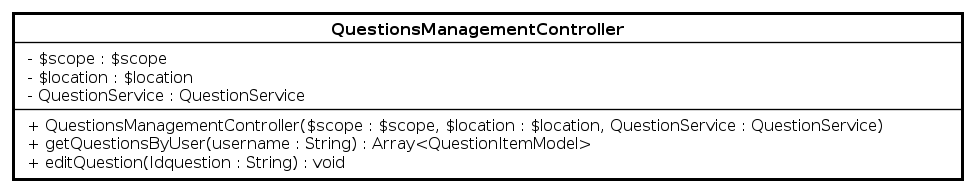
\includegraphics[scale=0.45]{UML/Classi/Front-End/QuizziPedia_Front-end_Controller_QuestionsManagementController.png}
	\caption{QuizziPedia::Front-End::Controllers::QuestionsManagementController}
\end{figure} \FloatBarrier
\begin{itemize}
	\item \textbf{Descrizione}: questa classe permette di gestire le domande create dall'utente e di crearne di nuove;
	\item \textbf{Utilizzo}: fornisce le funzionalità per richiedere al server le domande create dall'utente e mostrarle nella pagina dedicata. Inoltre permette di catturare gli eventi per modificare le domande esistenti e per crearne una di nuova; 
	\item \textbf{Relazione con altre classi}:
	\begin{itemize}
		\item \textit{IN} \texttt{QuestionsManagementModelView}: classe di tipo modelview la cui istanzazione è contenuta all'interno della variabile di ambiente \$scope di \textit{Angular.js\ped{G}}. All'interno di essa sono presenti le variabili e i metodi necessari per il \textit{Two-Way Data-Binding\ped{G}} tra la view \texttt{QuestionsManagementView} e il controller \texttt{QuestionsManagementController}; 
		\item \textit{IN} \texttt{QuestionService}: questa classe permette di ottenere domande esistenti e salvare nuove domande;
	\end{itemize}
	\item \textbf{Attributi}:
	\begin{itemize}
		\item \texttt{-} \texttt{\$scope: \$scope} \\
		Campo dati contenente un riferimento all’oggetto \$scope creato da \textit{Angular\ped{G}}, viene utilizzato come mezzo di comunicazione tra il controller e la view. Contiene gli oggetti che definiscono il model dell’applicazione;
		\item \texttt{-} \texttt{\$location: \$location} \\
		Campo dati contenente un riferimento al servizio creato da \textit{Angular\ped{G}} che permette di accedere alla barra degli indirizzi del \textit{browser\ped{G}}, i cambiamenti all’URL nella barra degli indirizzi si riflettono in questo oggetto e viceversa;
		\item \texttt{-} \texttt{QuestionService}\\
		Campo dati contenente un riferimento al servizio che si occupa della gestione delle informazioni legate alle domande;
	\end{itemize}
	\item \textbf{Metodi}:
	\begin{itemize}
		\item \texttt{+} \texttt{QuestionsManagementsController(\$scope: \$scope, \$location: \$location, QuestionService: QuestionService)} \\ 
		Metodo costruttore della classe; \\
		\textbf{Parametri}:
		\begin{itemize}
			\item \texttt{\$scope: \$scope} \\
			Parametro contenente un riferimento all’oggetto \$scope creato da \textit{Angular\ped{G}}. Viene utilizzato come mezzo di comunicazione tra il controller e la view. Contiene gli oggetti che definiscono il viewmodel e il model dell’applicazione;
			\item \texttt{\$location: \$location} \\
			Parametro contenente un riferimento al servizio creato da \textit{Angular\ped{G}} che permette di accedere alla barra degli indirizzi del \textit{browser\ped{G}}, i cambiamenti all’URL nella barra degli indirizzi si riflettono in questo oggetto e viceversa;
			\item \texttt{QuestionService: QuestionService} \\
			Parametro contenente un riferimento al servizio che si occupa della gestione delle informazioni legate alle domande;
		\end{itemize}
		\item \texttt{-} \texttt{getQuestionsByUser(username: String)} \\ 
		Metodo che acquisisce le domande create dall'utente attraverso il \texttt{QuestionService};\\
		\textbf{Parametri}:
		\begin{itemize}
			\item \texttt{username: String} \\
			Parametro di tipo \texttt{String} contenente l'username dell'utente;
		\end{itemize}
		\item \texttt{+} \texttt{editQuestion(idQuestion: String)} \\ 
		Metodo che gestisce l’evento click sul pulsante per modificare la domanda. Effettua il redirect alla pagina di modifica della domanda. \\
		\textbf{Parametri}:
		\begin{itemize}
			\item \texttt{idQuestion: username} \\
			Parametro di tipo \texttt{String} contenente l'id della domanda da modificare;
		\end{itemize}
	\end{itemize}
\end{itemize}

\paragraph{QuizziPedia::Front-End::Controllers::NewQuestionsButtonController}
\begin{figure} [ht]
	\centering
	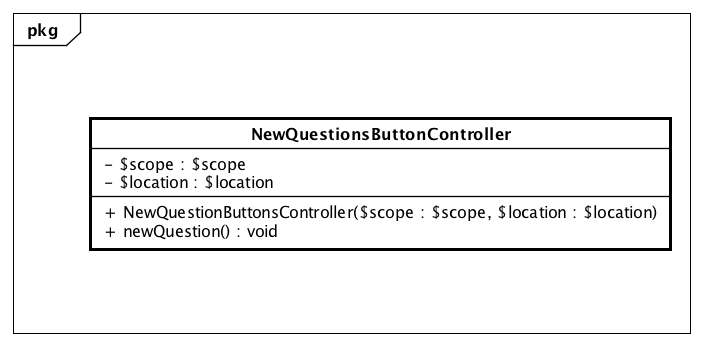
\includegraphics[scale=0.45]{UML/Classi/Front-End/QuizziPedia_Front-end_Controller_NewQuestionsButtonController.png}
	\caption{QuizziPedia::Front-End::Controllers::NewQuestionButtonController}
\end{figure} \FloatBarrier
\begin{itemize}
	\item \textbf{Descrizione}: questa classe permette di effettuare il redirect alla pagina di creazione nuova domanda;
	\item \textbf{Utilizzo}: effettua il redirect alla pagina di creazione di una nuova domanda quando l'utente seleziona interagisce con il bottone a cui è collegato il corrispettivo evento;
	\item \textbf{Relazione con altre classi}:
	\begin{itemize}
		\item \textit{IN} \texttt{NewQuestionButtonsModelView}: classe di tipo modelview la cui istanzazione è contenuta all'interno della variabile di ambiente \$scope di \textit{Angular.js\ped{G}}. All'interno di essa sono presenti le variabili e i metodi necessari per il \textit{Two-Way Data-Binding\ped{G}} tra la directive \texttt{NewQuestionButtonsDirective} e il controller \texttt{NewQuestionsButtonController}; 
	\end{itemize}
	\item \textbf{Attributi}:
	\begin{itemize}
		\item \texttt{-} \texttt{\$scope: \$scope} \\
		Campo dati contenente un riferimento all’oggetto \$scope creato da \textit{Angular\ped{G}}, viene utilizzato come mezzo di comunicazione tra il controller e la view. Contiene gli oggetti che definiscono il model dell’applicazione;
		\item \texttt{-} \texttt{\$location: \$location} \\
		Campo dati contenente un riferimento al servizio creato da \textit{Angular\ped{G}} che permette di accedere alla barra degli indirizzi del \textit{browser\ped{G}}, i cambiamenti all’URL nella barra degli indirizzi si riflettono in questo oggetto e viceversa;
	\end{itemize}
	\item \textbf{Metodi}:
	\begin{itemize}
		\item \texttt{+} \texttt{NewQuestionButtonsController(\$scope: \$scope, \$location: \$location)} \\ 
		Metodo costruttore della classe. \\
		\textbf{Parametri}:
		\begin{itemize}
			\item \texttt{\$scope: \$scope} \\
			Parametro contenente un riferimento all’oggetto \$scope creato da \textit{Angular\ped{G}}. Viene utilizzato come mezzo di comunicazione tra il controller e la view. Contiene gli oggetti che definiscono il viewmodel e il model dell’applicazione;
			\item \texttt{\$location: \$location} \\
			Parametro contenente un riferimento al servizio creato da \textit{Angular\ped{G}} che permette di accedere alla barra degli indirizzi del \textit{browser\ped{G}}, i cambiamenti all’URL nella barra degli indirizzi si riflettono in questo oggetto e viceversa;
		\end{itemize}
		\item \texttt{+} \texttt{newQuestion()} \\ 
		Metodo che gestisce l’evento click sul pulsante per creare una nuova domanda. Effettua il redirect alla pagina di creazione di una domanda;
	\end{itemize}
	
\end{itemize}

\paragraph{QuizziPedia::Front-End::Controllers::StatisticsController}
\begin{figure} [ht]
	\centering
	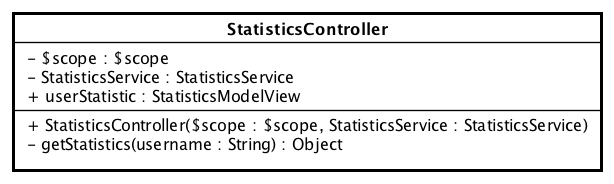
\includegraphics[scale=0.45]{UML/Classi/Front-End/QuizziPedia_Front-end_Controller_StatisticsController.png}
	\caption{QuizziPedia::Front-End::Controllers::StatisticsController}
\end{figure} \FloatBarrier
\begin{itemize}
	\item \textbf{Descrizione}: questa classe permette di le statistiche di un utente;
	\item \textbf{Utilizzo}: fornisce le funzionalità per ottenere le statistiche di un utente per poterle mostrare nella view;
	\item \textbf{Relazione con altre classi}:
	\begin{itemize}
		\item \textit{IN} \texttt{StatisticsModelView}: classe di tipo modelview la cui istanzazione è contenuta all'interno della variabile di ambiente \$scope di \textit{Angular.js\ped{G}}. All'interno di essa sono presenti le variabili e i metodi necessari per il \textit{Two-Way Data-Binding\ped{G}} tra la directive \texttt{StatisticsDirective} e il controller \texttt{StatisticsController}; 
		\item \textit{IN} \texttt{StatisticsService}: questa classe permette di ottenere le statistiche dell'utente;
	\end{itemize}
	\item \textbf{Attributi}:
	\begin{itemize}
		\item \texttt{-} \texttt{\$scope: \$scope} \\
		Campo dati contenente un riferimento all’oggetto \$scope creato da \textit{Angular\ped{G}}, viene utilizzato come mezzo di comunicazione tra il controller e la view. Contiene gli oggetti che definiscono il model dell’applicazione;
		\item \texttt{-} \texttt{StatisticsService: StatisticsService} \\
		Campo dati contenente un riferimento al servizio che si occupa della gestione delle informazioni legate alle statistiche da visualizzare;
	\end{itemize}	
	\begin{itemize}
		\item \textbf{Metodi}:
		\item \texttt{+} \texttt{StatisticsController(\$scope: \$scope, StatisticsService: StatisticsService)} \\ 
		Metodo costruttore della classe. \\
		\begin{itemize}
			\item \texttt{\$scope: \$scope} \\
			Parametro contenente un riferimento all’oggetto \$scope creato da \textit{Angular\ped{G}}. Viene utilizzato come mezzo di comunicazione tra il controller e la view. Contiene gli oggetti che definiscono il viewmodel e il model dell’applicazione;
			\item \texttt{StatisticsService: StatisticsService} \\
			Parametro contenente un riferimento al servizio che si occupa della gestione delle informazioni legate alle statistiche da visualizzare;
		\end{itemize}
		\item \texttt{-} \texttt{getStatistics(username: String)} \\ 
		Metodo che permette di ottenere le statistiche si un utente grazie all'utilizzo di \texttt{StatisticsService}; \\
		\textbf{Parametri}: 
		Metodo costruttore della classe. \\
		\begin{itemize}
			\item \texttt{username: String} \\
			Parametro contenente la stringa username utilizzata per poter recuperare le giuste statistiche attraverso lo \texttt{StatisticsService}; 
		\end{itemize}
	\end{itemize}
\end{itemize}

\paragraph{QuizziPedia::Front-End::Controllers::MenuBarController}
\begin{figure} [ht]
	\centering
	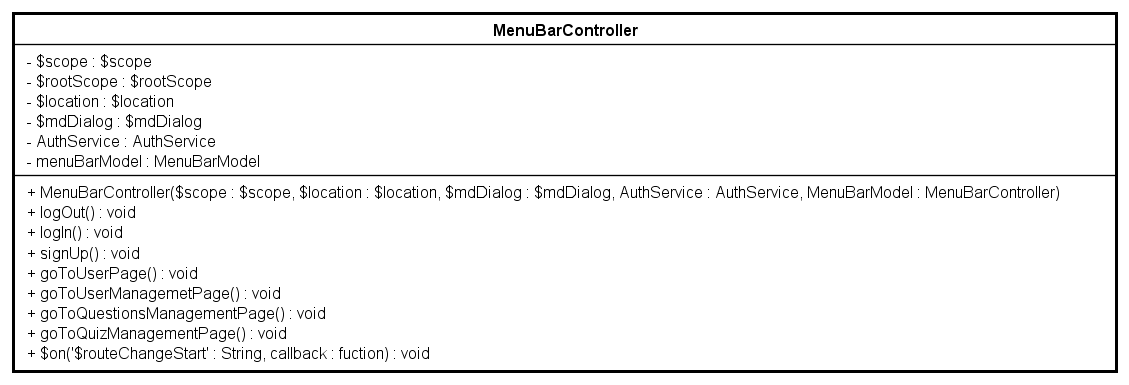
\includegraphics[scale=0.45]{UML/Classi/Front-End/QuizziPedia_Front-end_Controller_MenuBarController.png}
	\caption{QuizziPedia::Front-End::Controllers::MenuBarController}
\end{figure} \FloatBarrier
\begin{itemize}
	\item \textbf{Descrizione}: questa classe permette di gestire il menù fisso per ogni pagina;
	\item \textbf{Utilizzo}: fornisce le funzionalità per aggiornare, a seconda della pagina, il contenuto del menù;
	\item \textbf{Relazione con altre classi}:
	\begin{itemize}
		\item \textit{IN} \texttt{MenuBarModelView}: classe di tipo modelview la cui istanzazione è contenuta all'interno della variabile di ambiente \$scope di \textit{Angular.js\ped{G}}. All'interno di essa sono presenti le variabili e i metodi necessari per il \textit{Two-Way Data-Binding\ped{G}} tra la directive \texttt{MenuBarDirective} e il controller \texttt{MenuBarController}. Rappresenta il menù, presente in ogni pagina dell'applicazione, generato in base agli oggetti passati nello \$scope. Fornisce un pulsante per ogni oggetto ricevuto come parametro, ogni pulsante viene rappresentato con un’icona e con un testo. Al click di un pulsante viene invocata la funzione ad esso associata; 
		\item \textit{IN} \texttt{AuthService}: questa classe permette di gestire la registrazione e l'autenticazione di un utente;
		\item \textit{IN} \texttt{MenuBarModel}: questa classe rappresenta la classe che contiene le informazioni per la giusta visualizzazione della barra;
	\end{itemize}
	\item \textbf{Attributi}:
	\begin{itemize}
		\item \texttt{-} \texttt{\$scope: \$scope} \\
		Campo dati contenente un riferimento all’oggetto \$scope creato da \textit{Angular\ped{G}}, viene utilizzato come mezzo di comunicazione tra il controller e la view. Contiene gli oggetti che definiscono il model dell’applicazione;
		\item \texttt{-} \texttt{\$location: \$location} \\
		Campo dati contenente un riferimento al servizio creato da \textit{Angular\ped{G}} che permette di accedere alla barra degli indirizzi del \textit{browser\ped{G}}, i cambiamenti all’URL nella barra degli indirizzi si riflettono in questo oggetto e viceversa; 
		\item \texttt{-} \texttt{\$mdDialog: \$mdDialog} \\
		Campo dati contenente un riferimento al servizio della libreria \textit{Material for Angular\ped{G}} che permette di creare delle componenti a popup;
		\item \texttt{-} \texttt{AuthService: AuthService} \\
		Campo dati contenente un riferimento al servizio che si occupa della gestione delle informazioni legate all’autenticazione;
		\item \texttt{-} \texttt{MenuBarModel: MenuBarModel}: \\
		Campo dati contenente un riferimento all'oggetto che contiene le informazioni per la giusta visualizzazione della barra;
		
	\end{itemize}
	\item \textbf{Metodi}:
	\begin{itemize}
		\item \texttt{+} \texttt{MenuBarController(\$scope: \$scope, \$location: \$location, \$mdDialog: \$mdDialog, AuthService: AuthService, MenuBarModel: MenuBarModel)} \\
		Metodo costruttore della classe; \\
		\textbf{Parametri}:
		\begin{itemize}
			\item \texttt{\$scope: \$scope} \\
			Parametro contenente un riferimento all’oggetto \$scope creato da \textit{Angular\ped{G}}. Viene utilizzato come mezzo di comunicazione tra il controller e la view. Contiene gli oggetti che definiscono il viewmodel e il model dell’applicazione;
			\item \texttt{\$location: \$location} \\
			Parametro contenente un riferimento al servizio creato da \textit{Angular\ped{G}} che permette di accedere alla barra degli indirizzi del \textit{browser\ped{G}}, i cambiamenti all’URL nella barra degli indirizzi si riflettono in questo oggetto e viceversa;
			\item \texttt{\$mdDialog: \$mdDialog} \\
			Parametro contenente un riferimento al servizio della libreria \textit{Material for Angular\ped{G}} che permette di creare delle componenti a popup;
			\item \texttt{AuthService: AuthService} \\
			Parametro contenente un riferimento al servizio che si occupa della gestione delle informazioni legate all’autenticazione.  Viene utilizzato il metodo \texttt{logOut} di \$texttt{AuthService} a cui viene passato il parametro \texttt{username};
			\item \texttt{MenuBarModel: MenuBarModel}: \\
			Parametro contenente un riferimento all'oggetto che contiene le informazioni per la giusta visualizzazione della barra;
		\end{itemize}
		\item \texttt{+} \texttt{logOut(): void} \\
		Metodo che richiama il metodo \texttt{logOut} del service \texttt{AuthService} passandogli lo \texttt{username}. Prima di effettuare questa operazione viene mostrato a video un messaggio di conferma per il proseguo dell'operazione; 
		\item \texttt{+} \texttt{logIn(): void} \\
		Metodo che gestisce l’evento click sul pulsante per effettuare il login. Effettua il redirect alla pagina per effettuare il login; 
		\item \texttt{+} \texttt{signUp(): void} \\
		Metodo che gestisce l’evento click sul pulsante per effettuare la registrazione. Effettua il redirect alla pagina per effettuare la registrazione; 
		\item \texttt{+} \texttt{goToUserPage(): void} \\
		Metodo che gestisce l’evento click sul pulsante di visualizzazione della pagina utente. Effettua il redirect alla pagina di visualizzazione della pagina utente; 
		\item \texttt{+} \texttt{goToUserManagemetPage(): void} \\
		Metodo che gestisce l’evento click sul pulsante di gestione del profilo utente. Effettua il redirect alla pagina di gestione del profilo utente; 
		\item \texttt{+} \texttt{goToQuestionsManagementPage(): void} \\
		Metodo che gestisce l’evento click sul pulsante di gestione delle domande. Effettua il redirect alla pagina di gestione delle domande; 
		\item \texttt{+} \texttt{goToQuizManagementPage(): void} \\
		Metodo che gestisce l’evento click sul pulsante di gestione dei questionari. Effettua il redirect alla pagina di gestione dei questionari; 
	\end{itemize}
	
\end{itemize}
\paragraph{QuizziPedia::Front-End::Controllers::TrainingController}
\begin{figure} [ht]
	\centering
	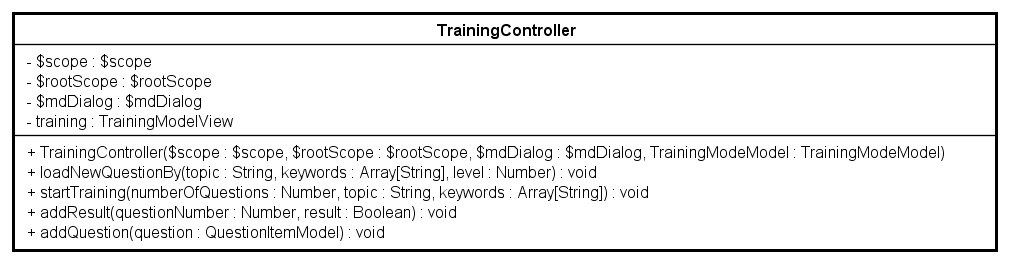
\includegraphics[scale=0.45]{UML/Classi/Front-End/QuizziPedia_Front-end_Controller_TrainingController.png}
	\caption{QuizziPedia::Front-End::Controllers::TrainingController}
\end{figure} \FloatBarrier
\begin{itemize}
	\item \textbf{Descrizione}: questa classe permette di gestire la modalità allenamento sottoponendo all'utente le giuste domande adatte al suo livello;
	\item \textbf{Utilizzo}: fornisce le funzionalità per recuperare le domande che siano in accordo con il livello dell'utente;
	\item \textbf{Relazione con altre classi}:
	\begin{itemize}
		\item \textit{IN} \texttt{TrainingModelView}: ;
		\item \textit{IN} \texttt{TrainingModeModel}: ;
		\item \textit{IN} \texttt{TrainingSetUpTemplate}: rappresenta il componente grafico che permette all'utente di selezionare l'argomento e le parole chiave per iniziare un allenamento con queste caratteristiche. Viene gestito dinamicamente all'interno della view TrainingView attraverso il controller TrainingController;
		\item \textit{IN} \texttt{QuestionController}: ;
		\item \textit{IN} \texttt{QuestionItemMode}: ;
	\end{itemize}
	\item \textbf{Attributi}:
	\begin{itemize}
		\item \texttt{-} \texttt{\$scope: \$scope} \\
		Campo dati contenente un riferimento all’oggetto \$scope creato da \textit{Angular\ped{G}}, viene utilizzato come mezzo di comunicazione tra il controller e la view. Contiene gli oggetti che definiscono il model dell’applicazione;
		\item \texttt{-} \texttt{\$rootScope: \$rootScope} \\
		Campo dati contenente il riferimento all'oggetto globale \$rootScope creato da \textit{Angular\ped{G}}. Viene utilizzato per rendere accessibile a tutti i controller e a tutte le view l'oggetto \texttt{TrainingModeModel}. In questo caso viene utilizzato per inserire in \$rootScope l'oggetto di ritorno della chiamata a \texttt{getNextQuestion};
		\item \texttt{-} \texttt{\$mdDialog: \$mdDialog} \\
		Campo dati contenente un riferimento al servizio della libreria \textit{Material for Angular\ped{G}} che permette di creare delle componenti a popup;
		\item \texttt{+} \texttt{training: TrainingModelView} \\
		Oggetto di tipo \texttt{TrainingModelView}. All'interno di esso sono presenti le variabili e i metodi necessari per il \textit{Two-Way Data-Binding\ped{G}} tra la view \texttt{TrainingView} e il controller \texttt{TrainingController};
	\end{itemize}
	\item \textbf{Metodi}:
	\begin{itemize}
		\item \texttt{+} \texttt{TrainingController(\$scope: \$scope, \$rootscope: \$rootscope, \$mdDialog: \$mdDialog)} \\ Metodo costruttore della classe; \\
		\textbf{Parametri:}
		\begin{itemize}
			\item \texttt{\$scope: \$scope} \\
			Parametro contenente un riferimento all’oggetto \$scope creato da \textit{Angular\ped{G}}. Viene utilizzato come mezzo di comunicazione tra il controller e la view. Contiene gli oggetti che definiscono il viewmodel e il model dell’applicazione;
			\item \texttt{\$rootscope: \$rootscope}\\
			Parametro contenente il riferimento all'oggetto globale \$rootScope creato da \textit{Angular\ped{G}}. Viene utilizzato per rendere accessibile a tutti i controller e a tutte le view l'oggetto \texttt{UserDetailsModel}. In questo caso viene utilizzato per aggiornare in \$rootScope l'oggetto che rappresenta l'utente autenticato all'interno dell'applicazione;
			\item \texttt{\$mdDialog: \$mdDialog} \\
			Parametro contenente un riferimento al servizio della libreria \textit{Material for Angular\ped{G}} che permette di creare delle componenti a popup.
		\end{itemize}
		\item \texttt{-} \texttt{getNextQuestion(): QuestionItemModel} \\ Metodo che gestisce l'evento del click al pulsante "prossima domanda", fa una richiesta al QuestionController che ritornerà la domanda successiva. Questa domanda andrà salvata nel TrainingModeModel nello \$scope.
	\end{itemize}
\end{itemize}

\paragraph{QuizziPedia::Front-End::Controllers::FillingQuestionnaireController}
\begin{figure} [ht]
	\centering
	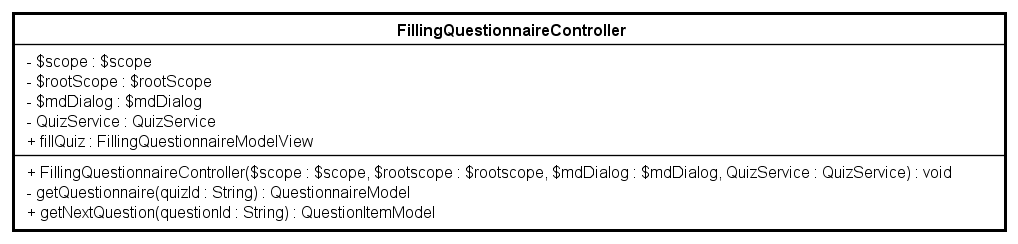
\includegraphics[scale=0.45]{UML/Classi/Front-End/QuizziPedia_Front-end_Controller_FillingQuestionnaireController.png}
	\caption{QuizziPedia::Front-End::Controllers::FillingQuestionnaireController}
\end{figure} \FloatBarrier
\begin{itemize}
	\item \textbf{Descrizione}: questa classe permette di gestire la compilazione del questionario;
	\item \textbf{Utilizzo}: fornisce le funzionalità per compilare un questionario e per gestire il cambio di domanda;
	\item \textbf{Relazione con altre classi}:
	\begin{itemize}
		\item \textit{IN} \texttt{FillingQuestionnaireModelView}: ;  
		\item \textit{IN} \texttt{InfoQuestionnaireTemplate}: rappresenta il componente grafico che permette all'utente di visualizzare le informazioni principali del questionario che si sta per svolgere. Viene gestito dinamicamente all'interno della view TrainingView attraverso il controller TrainingController;
		\item \textit{IN} \texttt{QuizService}: permette di ottenere i dati di un quiz tramite delle parole chiave inserite dall'utente nella barra di ricerca. Permette inoltre di iscriversi ad un questionario e di scaricare l'intera l'ista di domande di un questionario a partire dal suo id univoco;
		\item \textit{IN} \texttt{QuestionnaireModel}: ;
		\item \textit{IN} \texttt{QuestionsController}: ; 
		\item \textit{IN} \texttt{QuestionItemModel}: ;
	\end{itemize}
	\item \textbf{Attributi}:
	\begin{itemize}
		\item \texttt{-} \texttt{\$scope: \$scope} \\
		Campo dati contenente un riferimento all’oggetto \$scope creato da \textit{Angular\ped{G}}, viene utilizzato come mezzo di comunicazione tra il controller e la view. Contiene gli oggetti che definiscono il model dell’applicazione;
		\item \texttt{-} \texttt{\$rootScope: \$rootScope} \\
		Campo dati contenente il riferimento all'oggetto globale \$rootScope creato da \textit{Angular\ped{G}}. Viene utilizzato per rendere accessibile a tutti i controller e a tutte le view l'oggetto \texttt{QuestionnaireModel}. In questo caso viene utilizzato per inserire in \$rootScope l'oggetto di ritorno della chiamata a \texttt{getNextQuestion} e l'intero questionario ritornato dalla chiamata a \texttt{getQuestionnaire};
		\item \texttt{-} \texttt{\$mdDialog: \$mdDialog} \\
		Campo dati contenente un riferimento al servizio della libreria \textit{Material for Angular\ped{G}} che permette di creare delle componenti a popup;
		\item \texttt{-} \texttt{QuizService: QuizService}: ;
		\item \texttt{+} \texttt{fillQuiz: FillingQuestionnaireModelView} \\
		Oggetto di tipo \texttt{FillingQuestionnaireModelView}. All'interno di esso sono presenti le variabili e i metodi necessari per il \textit{Two-Way Data-Binding\ped{G}} tra la view \texttt{FillingQuestionnaireView} e il controller \texttt{FillingQuestionnaireController};
	\end{itemize}
	\item \textbf{Metodi}:
	\begin{itemize}
		\item \texttt{+} \texttt{FillingQuestionnaireController(\$scope: \$scope, \$rootscope: \$rootscope, \$mdDialog: \$mdDialog, QuizService: QuizService)} \\Metodo costruttore della classe.\\
		\textbf{Parametri}:
		\begin{itemize}
			\item \texttt{-} \texttt{\$scope: \$scope} \\
			Campo dati contenente un riferimento all’oggetto \$scope creato da \textit{Angular\ped{G}}. Viene utilizzato come mezzo di comunicazione tra il controller e la view. Contiene gli oggetti che definiscono il viewmodel e il model dell’applicazione;
			\item \texttt{-} \texttt{\$location: \$location} \\
			Campo dati contenente un riferimento al servizio creato da \textit{Angular\ped{G}} che permette di accedere alla barra degli indirizzi del \textit{browser\ped{G}}, i cambiamenti all’URL nella barra degli indirizzi si riflettono in questo oggetto e viceversa;
			\item \texttt{-} \texttt{\$mdDialog: \$mdDialog} \\
			Campo dati contenente un riferimento al servizio della libreria \textit{Material for Angular\ped{G}} che permette di creare delle componenti a popup;
			\item \texttt{QuizService: QuizService}: parametro che permette di ottenere, tramite il service, la lista di tutte le domande presenti nel quiz;
		\end{itemize}
		\item \texttt{+} \texttt{getQuestionnaire(quizId: String): QuestionnaireModel}: \\ Metodo che permette di ottenere l'intero questionario; \\
		\textbf{Parametri}:
		\begin{itemize}
			\item \texttt{quizId: String}: parametro che indica l'id del quiz che vogliamo ricevere dal back-end.
		\end{itemize}
		\item \texttt{+} \texttt{getNextQuestion(questionId: String): QuestionItemModel}: \\ Metodo che ritorna la domanda successiva del quiz tramite chiamata a QuestionController; \\
		\textbf{Parametri}:
		\begin{itemize}
			\item \texttt{questionId: String}: parametro che indica l'id della domanda che vogliamo ricevere dal back-end.
		\end{itemize}
	\end{itemize}
\end{itemize}

\paragraph{QuizziPedia::Front-End::Controllers::CreateQuestionnaireController}
\begin{figure} [ht]
	\centering
	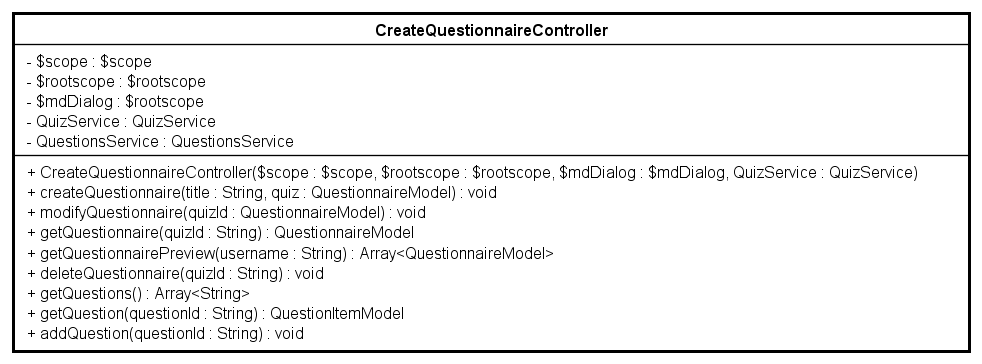
\includegraphics[scale=0.45]{UML/Classi/Front-End/QuizziPedia_Front-end_Controller_CreateQuestionnaireController.png}
	\caption{QuizziPedia::Front-End::Controllers::CreateQuestionnaireController}
\end{figure} \FloatBarrier
\begin{itemize}
	\item \textbf{Descrizione}: questa classe permette di gestire la creazione di un questionario;
	\item \textbf{Utilizzo}: fornisce tutte le funzionalità per la creazione di un nuovo questionario e per la modifica di uno esistente;
	\item \textbf{Relazione con altre classi}:
	\begin{itemize}
		\item \textit{IN} \texttt{CreateQuestionnaireModelView}: view per la creazione del questionario; 
		\item \textit{IN} \texttt{QuizService}: questa classe permette di ottenere i dati di un quiz tramite delle parole chiave inserite dall'utente nella barra di ricerca;
		\item \textit{IN} \texttt{QuestionnaireModel}: ;
	\end{itemize}
	\item \textbf{Attributi}:
	\begin{itemize}
		\item \texttt{-} \texttt{\$scope: \$scope} \\
		Campo dati contenente un riferimento all’oggetto \$scope creato da \textit{Angular\ped{G}}, viene utilizzato come mezzo di comunicazione tra il controller e la view. Contiene gli oggetti che definiscono il model dell’applicazione;
		\item \texttt{-} \texttt{\$rootScope: \$rootScope} \\
		Campo dati contenente il riferimento all'oggetto globale \$rootScope creato da \textit{Angular\ped{G}}. Viene utilizzato per rendere accessibile a tutti i controller e a tutte le view l'oggetto \texttt{QuestionnaireModel}. In questo caso viene utilizzato per inserire in \$rootScope l'oggetto di ritorno della chiamata a \texttt{getQuestiontionnaire} e la lista dei questionari ottenuta dalla chiamata \texttt{getQuestionnairePreview};
		\item \texttt{-} \texttt{\$mdDialog: \$mdDialog} \\
		Campo dati contenente un riferimento al servizio della libreria \textit{Material for Angular\ped{G}} che permette di creare delle componenti a popup;
		\item \texttt{-} \texttt{QuizService}: ;
	\end{itemize}
	\item \textbf{Metodi}:
	\begin{itemize}
		\item \texttt{+} \texttt{CreateQuestionnaireController(\$scope: \$scope, \$rootscope: \$rootscope, \$mdDialog: \$mdDialog, QuizService: QuizService)}: \\ Metodo costruttore della classe. \\
		\textbf{Parametri}:
		\begin{itemize}
			\item \texttt{-} \texttt{\$scope: \$scope} \\
			Campo dati contenente un riferimento all’oggetto \$scope creato da \textit{Angular\ped{G}}. Viene utilizzato come mezzo di comunicazione tra il controller e la view. Contiene gli oggetti che definiscono il viewmodel e il model dell’applicazione;
				\item \texttt{-} \texttt{\$rootScope: \$rootScope} \\
				Campo dati contenente il riferimento all'oggetto globale \$rootScope creato da \textit{Angular\ped{G}}. Viene utilizzato per rendere accessibile a tutti i controller e a tutte le view l'oggetto \texttt{QuestionnaireModel}. In questo caso viene utilizzato per inserire in \$rootScope l'oggetto di ritorno della chiamata a \texttt{getQuestiontionnaire} e la lista dei questionari ottenuta dalla chiamata \texttt{getQuestionnairePreview};
			\item \texttt{-} \texttt{\$mdDialog: \$mdDialog} \\
			Campo dati contenente un riferimento al servizio della libreria \textit{Material for Angular\ped{G}} che permette di creare delle componenti a popup;
			\item \texttt{QuizService: QuizService}: parametro che permette di ottenere, tramite il service, la lista di tutte le domande presenti nel quiz;
		\end{itemize}
		\item \texttt{+} \texttt{createQuestionnaire(title: String, quiz: QuestionnaireModel)}: \\Metodo che permette di inserire un questionario nel database tramite richiesta al service; \\
			\textbf{Parametri}:
			\begin{itemize}
				\item 
			\end{itemize}
		\item \texttt{+} \texttt{modifyQuestionnaire(quizId: QuestionnaireModel)}: \\ Metodo che serve per modificare un questionario; \\
			\textbf{Parametri}:
			\begin{itemize}
				\item \texttt{quiz: QuestionnaireModel}: parametro che rappresenta l'oggetto questionario;
			\end{itemize}
		\item \texttt{+} \texttt{getQuestionnaire(quizId: String)}: \\Metodo che serve per ottenere un questionario tramite l'id in modo da poterlo modificare; \\
			\textbf{Parametri}:
			\begin{itemize}
				\item \texttt{quizId: String}: parametro che rappresenta l'id del questionario da richiedere.
			\end{itemize}
		\item \texttt{+} \texttt{getQuestionnairePreview(username: String)}: \\ Metodo che serve per ottenere la lista di tutti i questionari di un utente; \\
			\textbf{Parametri}:
			\begin{itemize}
				\item \texttt{username: String}: parametro che indica l'utente del quale vogliamo caricare tutti i questionari.
			\end{itemize}
		\item \texttt{+} \texttt{deleteQuestionnaire(quizId: String): void}: \\Metodo che elimina un questionario.
		\textbf{Parametri}:
		\texttt{quizId: String}: identificativo del questionario da eliminare.
	\end{itemize}
\end{itemize}

\paragraph{QuizziPedia::Front-End::Controllers::RegistrationManagementController}
\begin{figure} [ht]
	\centering
	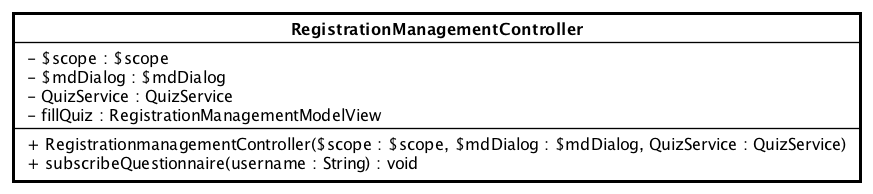
\includegraphics[scale=0.45]{UML/Classi/Front-End/QuizziPedia_Front-end_Controller_RegistrationManagementController.png}
	\caption{QuizziPedia::Front-End::Controllers::RegistrationManagementController}
\end{figure} \FloatBarrier
\begin{itemize}
	\item \textbf{Descrizione}: questa classe permette di gestire le iscrizione degli utenti ai questionari;
	\item \textbf{Utilizzo}: fornisce le funzionalità di iscrizione ad un questionario;
	\item \textbf{Relazione con altre classi}:
	\begin{itemize}
		\item \textit{IN} \texttt{RegistratioManagementModelView}: ; 
		\item \textit{OUT} \texttt{QuizService}: questa classe permette di ottenere i dati di un quiz tramite delle parole chiave inserite dall'utente nella barra di ricerca;
	\end{itemize}
	\item \textbf{Attributi}:
	\begin{itemize}
		\item \texttt{-} \texttt{\$scope: \$scope} \\
		Campo dati contenente un riferimento all’oggetto \$scope creato da \textit{Angular\ped{G}}, viene utilizzato come mezzo di comunicazione tra il controller e la view. Contiene gli oggetti che definiscono il model dell’applicazione;
		\item \texttt{-} \texttt{\$mdDialog: \$mdDialog} \\
		Campo dati contenente un riferimento al servizio della libreria \textit{Material for Angular\ped{G}} che permette di creare delle componenti a popup;
		\item \texttt{QuizService: QuizService}: parametro che permette di ottenere, tramite il service, la lista di tutte le domande presenti nel quiz;
	\end{itemize}
	\item \textbf{Metodi}:
	\begin{itemize}
		\item \texttt{RegistrationmanagementController(\$scope: \$scope, \$mdDialog: \$mdDialog, QuizService: QuizService)}: \\Metodo costruttore della classe. \\
			\textbf{Parametri}:
			\begin{itemize}
					\item \texttt{-} \texttt{\$scope: \$scope} \\
					Campo dati contenente un riferimento all’oggetto \$scope creato da \textit{Angular\ped{G}}. Viene utilizzato come mezzo di comunicazione tra il controller e la view. Contiene gli oggetti che definiscono il viewmodel e il model dell’applicazione;
					\item \texttt{-} \texttt{\$mdDialog: \$mdDialog} \\
					Campo dati contenente un riferimento al servizio della libreria \textit{Material for Angular\ped{G}} che permette di creare delle componenti a popup;
					\item \texttt{-} \texttt{QuizService: QuizService}: parametro che permette di ottenere, tramite il service, la lista di tutte le domande presenti nel quiz; 
			\end{itemize}
		\item \texttt{subscribeQuestionnaire(username: String): void} \\ Metodo che permette l'iscrizione ad un questionario. Richiama la funzionalità del QuizService. \\
		\textbf{Parametri}:
		\begin{itemize}
			\item \texttt{username: String}: parametro che indica l'utente da iscrivere al questionario.
		\end{itemize}
	\end{itemize}
\end{itemize}

\paragraph{QuizziPedia::Front-End::Controllers::ResultsController}
\begin{figure} [ht]
	\centering
	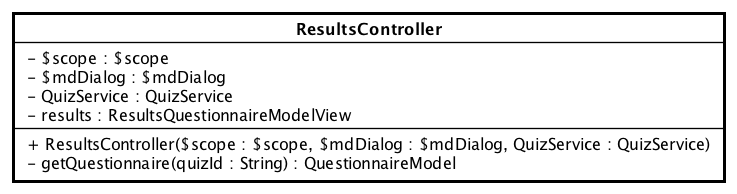
\includegraphics[scale=0.45]{UML/Classi/Front-End/QuizziPedia_Front-end_Controller_ResultsController.png}
	\caption{QuizziPedia::Front-End::Controllers::ResultsController}
\end{figure} \FloatBarrier
\begin{itemize}
	\item \textbf{Descrizione}: questa classe permette di gestire i risultati della ricerca effettuata dall'utente;
	\item \textbf{Utilizzo}: fornisce le funzionalità per recuperare i dati dal back-end e mostrarli all'utente nella view;
	\item \textbf{Relazione con altre classi}:
	\begin{itemize}
		\item \textit{IN} \texttt{ResultsQuestionnaireModelView}: ; 
		\item \textit{IN} \texttt{QuizService}: questa classe permette di ottenere i dati di un quiz tramite delle parole chiave inserite dall'utente nella barra di ricerca;
		\item \textit{IN} \texttt{QuestionnaireModel}: ;
	\end{itemize}
	\item \textbf{Attributi}:
	\begin{itemize}
		\item \texttt{-} \texttt{\$scope: \$scope} \\
		Campo dati contenente un riferimento all’oggetto \$scope creato da \textit{Angular\ped{G}}, viene utilizzato come mezzo di comunicazione tra il controller e la view. Contiene gli oggetti che definiscono il model dell’applicazione;
		\item \texttt{-} \texttt{\$mdDialog: \$mdDialog} \\
		Campo dati contenente un riferimento al servizio della libreria \textit{Material for Angular\ped{G}} che permette di creare delle componenti a popup;
		\item \textit{-} \texttt{QuizService}: questa classe permette di ottenere i dati di un quiz tramite delle parole chiave inserite dall'utente nella barra di ricerca;
	\end{itemize}
	\item \textbf{Metodi}:
	\begin{itemize}
		\item \texttt{+} \texttt{ResultsController(\$scope: \$scope, \$mdDialog: \$mdDialog), QuizService: QuizService}: \\Metodo costruttore della classe. \\
		\textbf{Parametri}: 
		\begin{itemize}
			\item \texttt{-} \texttt{\$scope: \$scope} \\
			Campo dati contenente un riferimento all’oggetto \$scope creato da \textit{Angular\ped{G}}. Viene utilizzato come mezzo di comunicazione tra il controller e la view. Contiene gli oggetti che definiscono il viewmodel e il model dell’applicazione;
			\item \texttt{-} \texttt{\$mdDialog: \$mdDialog} \\
			Campo dati contenente un riferimento al servizio della libreria \textit{Material for Angular\ped{G}} che permette di creare delle componenti a popup;
			\item \texttt{-} \texttt{QuizService: QuizService}: parametro che permette di ottenere, tramite il service, la lista di tutte le domande presenti nel quiz;
		\end{itemize}
		\item \texttt{-} \texttt{getQuestionnaire(quizId: String): QuestionnaireModel}: \\Metodo che ritorna tutti i dati di un questionario.\\
		\textbf{Parametri}:
		\begin{itemize}
			\item \texttt{quizId: String}: parametro che indica l'id univoco del questionario da caricare.
		\end{itemize}
	\end{itemize}
\end{itemize}

\paragraph{QuizziPedia::Front-End::Controllers::QuestionnaireManagementController}
\begin{figure} [ht]
	\centering
	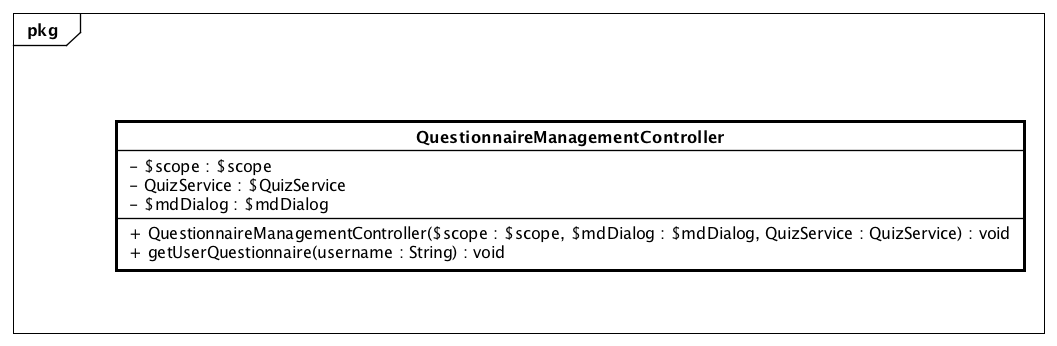
\includegraphics[scale=0.45]{UML/Classi/Front-End/QuizziPedia_Front-end_Controller_QuestionnaireManagementController.png}
	\caption{QuizziPedia::Front-End::Controllers::QuestionnaireManagementController}
\end{figure} \FloatBarrier
\begin{itemize}
	\item \textbf{Descrizione}: questa classe permette di gestire tutti i questionari creati da un utente; 
	\item \textbf{Utilizzo}: fornisce le funzionalità per recuperare dal back-end tutti i questionari creati da un utente;
	\item \textbf{Relazione con altre classi}:
	\begin{itemize}
		\item \textit{IN} \texttt{QuestionnaireManagementeModelView}: ;
		\item \textit{IN} \texttt{QuizService}: questa classe permette di ottenere i dati di un quiz tramite delle parole chiave inserite dall'utente nella barra di ricerca;
		\item \texttt{-} \texttt{\$mdDialog: \$mdDialog} \\
		Campo dati contenente un riferimento al servizio della libreria \textit{Material for Angular\ped{G}} che permette di creare delle componenti a popup;
		\item \textit{IN} \texttt{QuestionnaireModel}: ;
	\end{itemize}
	\item \textbf{Attributi}:
	\begin{itemize}
		\item \texttt{-} \texttt{\$scope: \$scope} \\
		Campo dati contenente un riferimento all’oggetto \$scope creato da \textit{Angular\ped{G}}, viene utilizzato come mezzo di comunicazione tra il controller e la view. Contiene gli oggetti che definiscono il model dell’applicazione;
		\item \textit{IN} \texttt{QuizService}: permette di ottenere i dati di un quiz tramite delle parole chiave inserite dall'utente nella barra di ricerca;
	\end{itemize}
	\item \textbf{Metodi}:
	\begin{itemize}
		\item \texttt{+} \texttt{QuestionnaireManagementController(\$scope: \$scope, \$mdDialog: \$mdDialog, QuizService: QuizService)}: \\Metodo costruttore della classe;\\
		\textbf{Parametri}: 
		\begin{itemize}
			\item \texttt{-} \texttt{\$scope: \$scope} \\
			Campo dati contenente un riferimento all’oggetto \$scope creato da \textit{Angular\ped{G}}. Viene utilizzato come mezzo di comunicazione tra il controller e la view. Contiene gli oggetti che definiscono il viewmodel e il model dell’applicazione;
			\item \texttt{-} \texttt{\$mdDialog: \$mdDialog} \\
			Campo dati contenente un riferimento al servizio della libreria \textit{Material for Angular\ped{G}} che permette di creare delle componenti a popup;
			\item \texttt{-} \texttt{QuizService: QuizService}: parametro che permette di ottenere, tramite il service, la lista di tutte le domande presenti nel quiz;
		\end{itemize}
		\item \texttt{-} \texttt{getUserQuestionnaire(username: String) QuestionnaireModel[]}: \\Metodo che ritorna tutti i questionari creati da un utente in un array di QuestionnaireModel.
		\textbf{Parametri}:
		\begin{itemize}
			\item \texttt{username: String}: parametro che indica l'identificativo dell'utente del quale vogliamo scaricare tutti i questionari.
		\end{itemize}
	\end{itemize}
\end{itemize}

\paragraph{QuizziPedia::Front-End::Controllers::QuestionnaireDetailsController}
\begin{figure} [ht]
	\centering
	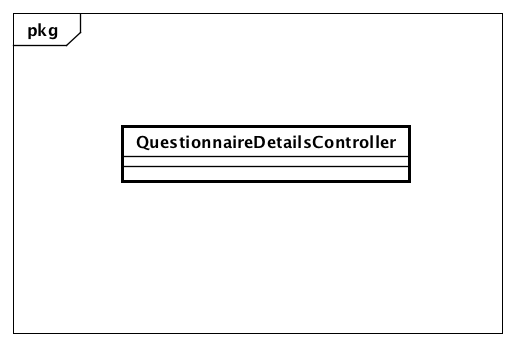
\includegraphics[scale=0.45]{UML/Classi/Front-End/QuizziPedia_Front-end_Controller_QuestionnaireDetailsController.png}
	\caption{QuizziPedia::Front-End::Controllers::QuestionnaireDetailsController}
\end{figure} \FloatBarrier
\begin{itemize}
	\item \textbf{Descrizione}: questa classe permette di gestire i dettagli di un questionario; 
	\item \textbf{Utilizzo}: fornisce le funzionalità per recuperare dal back-end i dettagli di un questionario creato da un utente al fine di poterli visualizzare nel suo profilo;
	\item \textbf{Relazione con altre classi}:
	\begin{itemize}
		\item \textit{IN} \texttt{QuestionnaireDetailsModelView}: ;
		\item \textit{IN} \texttt{QuizService}: questa classe permette di ottenere i dati di un quiz tramite delle parole chiave inserite dall'utente nella barra di ricerca;
		\item \textit{} \texttt{QuestionnaireModel}: ;
	\end{itemize}
	\item \textbf{Attributi}:
	\begin{itemize}
		\item \texttt{-} \texttt{\$scope: \$scope} \\
		Campo dati contenente un riferimento all’oggetto \$scope creato da \textit{Angular\ped{G}}, viene utilizzato come mezzo di comunicazione tra il controller e la view. Contiene gli oggetti che definiscono il model dell’applicazione;
		\item \texttt{-} \texttt{\$rootScope: \$rootScope} \\
		Campo dati contenente il riferimento all'oggetto globale \$rootScope creato da \textit{Angular\ped{G}}. Viene utilizzato per rendere accessibile a tutti i controller e a tutte le view l'oggetto \texttt{QuestionnaireModel}. In questo caso viene utilizzato per inserire in \$rootScope l'oggetto di ritorno della chiamata a \texttt{getQuestionnaireDetails} del service \texttt{QuizService};
		
	\end{itemize}
	\item \textbf{Metodi}:
	\begin{itemize}
		\item \texttt{+} \texttt{QuestionnaireDetailsController}: \\ Metodo costruttore della classe;
		\item \texttt{-} \texttt{getQuestionnaireDetails(username: String)}: \\ Metodo che richiede al service i dettagli dei questionari eseguiti dall'utente.
		\textbf{Parametri}:
		\begin{itemize}
			\item \texttt{username: String}: username dell'utente del quale caricare i questionari.
		\end{itemize}
		\item \texttt{-} \texttt{getSubscribedQuestionnaire(username: String)}: \\Metodo che ritorna i questionari a cui l'utente è iscritto.
		\textbf{Parametri}:
		\begin{itemize}
			\item \texttt{username: String}: identificativo dell'utente del quale scaricare i questionari a cui è iscritto.
		\end{itemize}
	\end{itemize}
\end{itemize}

\paragraph{QuizziPedia::Front-End::Controllers::UserDetailsController}
\begin{figure} [ht]
	\centering
	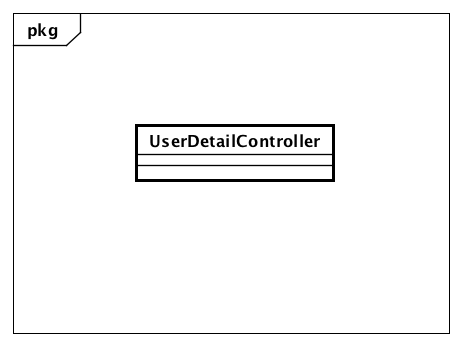
\includegraphics[scale=0.45]{UML/Classi/Front-End/QuizziPedia_Front-end_Controller_UserDetailController.png}
	\caption{QuizziPedia::Front-End::Controllers::UserDetailController}
\end{figure} \FloatBarrier
\begin{itemize}
	\item \textbf{Descrizione}: questa classe permette di ottenere i dati di un utente;
	\item \textbf{Utilizzo}: fornisce le funzionalità per ottenere i dati di un utente per poterle mostrare nella view;
	\item \textbf{Relazione con altre classi}:
	\begin{itemize}
		\item \textit{IN} \texttt{UserDetailsModelView}: directive che permette di visualizzare i dati di un utente; 
		\item \textit{IN} \texttt{UserDetailsService}: questa classe permette di ottenere i dati dell'utente;
		\item \textit{IN} \texttt{UserDetailsModel}: 
	\end{itemize}
	\item \textbf{Attributi}:
	\begin{itemize}
		\item \texttt{-} \texttt{\$scope: \$scope} \\
		Campo dati contenente un riferimento all’oggetto \$scope creato da \textit{Angular\ped{G}}, viene utilizzato come mezzo di comunicazione tra il controller e la view. Contiene gli oggetti che definiscono il model dell’applicazione;
		\item \texttt{-} \texttt{\$rootScope: \$rootScope} \\
		Campo dati contenente il riferimento all'oggetto globale \$rootScope creato da \textit{Angular\ped{G}}. Viene utilizzato per rendere accessibile a tutti i controller e a tutte le view l'oggetto \texttt{UserDetailsModel}. In questo caso viene utilizzato per inserire in \$rootScope l'oggetto di ritorno della chiamata a \texttt{getUserDetails} del service \texttt{UserDetailsService};
		\item \texttt{-} \texttt{userDetailsService}: parametro permette di ottenere i dati dell'utente;
	\end{itemize}	
	\begin{itemize}
		\item \textbf{Metodi}:
		\item \texttt{+} \texttt{UserDetailsController()} \\ Metodo costruttore della classe;
		\item \texttt{-} \texttt{getUserDetails(username: String)} \\ Metodo che permette di ottenere i dati con una chiamata a UserDetailsService;
	\end{itemize}
\end{itemize}

\paragraph{QuizziPedia::Front-End::Controllers::QuestionsController}
\begin{figure} [ht]
	\centering
	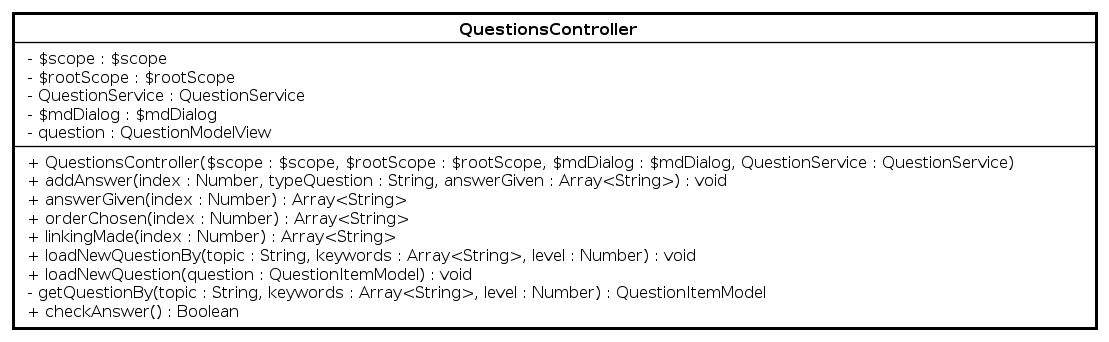
\includegraphics[scale=0.45]{UML/Classi/Front-End/QuizziPedia_Front-end_Controller_QuestionsController.png}
	\caption{QuizziPedia::Front-End::Controllers::QuestionsController}
\end{figure} \FloatBarrier
\begin{itemize}
	\item \textbf{Descrizione}: questa classe permette di gestire il recupero delle domande per poterle stampare nella modalità allenamento;
	\item \textbf{Utilizzo}: fornisce le funzionalità per il recupero delle domande esistenti nel database al fine di mostrarle durante la modalità allenamento nell'apposito template;
	\item \textbf{Relazione con altre classi}:
	\begin{itemize}
		\item \textit{IN} \texttt{HeaderTextQuestionTemplate}: rappresenta il componente grafico che presenta all'utente il testo della domanda, l'argomento e le parole chiave. Viene gestito dinamicamente all'interno della view TrainingView attraverso il controller TrainingController; 
		\item \textit{IN} \texttt{TrueFalseAnswerTemplate}: rappresenta il componente grafico che permette all'utente di visualizzare la domanda vero e falso. Viene gestito dinamicamente all'interno della view TrainingView attraverso il controller TrainingController; 
		\item \textit{IN} \texttt{MultipleChoiceAnswerTemplate}: rappresenta il componente grafico che permette all'utente di visualizzare la domanda a risposta multipla. Viene gestito dinamicamente all'interno della view TrainingView attraverso il controller TrainingController; 
		\item \textit{IN} \texttt{LinkingAnswerTemplate}: rappresenta il componente grafico che permette all'utente di visualizzare la domanda di collegamento. Viene gestito dinamicamente all'interno della view TrainingView attraverso il controller TrainingController; 
		\item \textit{IN} \texttt{SortImagesAnswerTemplate}: rappresenta il componente grafico che permette all'utente di visualizzare la domanda ad ordinamento di immagini. Viene gestito dinamicamente all'interno della view TrainingView attraverso il controller TrainingController; 
		\item \textit{IN} \texttt{SortTextAnswerTemplate}: rappresenta il componente grafico che permette all'utente di visualizzare la domanda ad ordinamento di stringhe. Viene gestito dinamicamente all'interno della view TrainingView attraverso il controller TrainingController; 
		\item \textit{IN} \texttt{EmptySpaceAnswerTemplate}: rappresenta il componente grafico che permette all'utente di visualizzare l'esercizio a riempimento di spazi vuoti. Viene gestito dinamicamente all'interno della view TrainingView attraverso il controller TrainingController; 
		\item \textit{IN} \texttt{ClickableAnswerTemplate}: rappresenta il componente grafico che permette all'utente di visualizzare la domanda ad area cliccabile nell'immagine. Viene gestito dinamicamente all'interno della view TrainingView attraverso il controller TrainingController;  
		\item \textit{IN} \texttt{QuestionServices}: questa classe permette di ottenere domande esistenti e salvare nuove domande;
		\item \textit{IN} \texttt{QuestionItemModel}: ;
		\item \textit{OUT} \texttt{FillingQuestionnaireController}: ;
		
	\end{itemize}
	\item \textbf{Attributi}:
	\begin{itemize}
		\item \texttt{-} \texttt{\$scope: \$scope} \\
		Campo dati contenente un riferimento all’oggetto \$scope creato da \textit{Angular\ped{G}}, viene utilizzato come mezzo di comunicazione tra il controller e la view. Contiene gli oggetti che definiscono il model dell’applicazione;
		\item \texttt{-} \texttt{\$rootScope: \$rootScope} \\
		Campo dati contenente il riferimento all'oggetto globale \$rootScope creato da \textit{Angular\ped{G}}. Viene utilizzato per rendere accessibile a tutti i controller e a tutte le view l'oggetto \texttt{QuestionItemModel}. In questo caso viene utilizzato per inserire in \$rootScope l'oggetto di ritorno della chiamata a \texttt{getQuestion} del service \texttt{QuestionService};
		\item \texttt{-} \texttt{QuestionService}: ;
	\end{itemize}
	\item \textbf{Metodi}:
	\begin{itemize}
		\item \texttt{+} \texttt{QuestionsController}: \\ Metodo costruttore della classe
		\item \texttt{+} \texttt{getQuestion}: \\ Metodo che richiede al back-end una domanda;
	\end{itemize}
\end{itemize}

\paragraph{QuizziPedia::Front-End::Controllers::TopicKeywordsController}
\begin{figure} [ht]
	\centering
	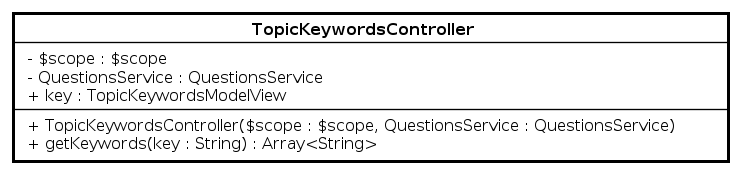
\includegraphics[scale=0.45]{UML/Classi/Front-End/QuizziPedia_Front-end_Controller_TopicKeywordsController.png}
	\caption{QuizziPedia::Front-End::Controllers::TopicKeywordsController}
\end{figure} \FloatBarrier
\begin{itemize}
	\item \textbf{Descrizione}: questa classe permette di gestire il recupero delle parole chiave di un questionario;
	\item \textbf{Utilizzo}: fornisce le funzionalità per il recupero delle parole chiave durante la creazione di un questionario;
	\item \textbf{Relazione con altre classi}:
	\begin{itemize}
		\item \textit{IN} \texttt{TopicKeywordsModelView}: directive che permette di gestire l'inserimento di keywords al momento della creazione della domanda; 
		\item \textit{IN} \texttt{QuestionsService}: questa classe permette di ottenere domande esistenti e salvare nuove domande;
	\end{itemize}
	\item \textbf{Attributi}:
	\begin{itemize}
		\item \texttt{-} \texttt{\$scope: \$scope} \\
		Campo dati contenente un riferimento all’oggetto \$scope creato da \textit{Angular\ped{G}}, viene utilizzato come mezzo di comunicazione tra il controller e la view. Contiene gli oggetti che definiscono il model dell’applicazione;
	\end{itemize}
	\item \textbf{Metodi}:
	\begin{itemize}
		\item \texttt{-} \texttt{getTopicKeywords(key: String)}: \\ Metodo che ritorna le parole che hanno a che fare con key
	\end{itemize}
\end{itemize}

\paragraph{QuizziPedia::Front-End::Controllers::QuestionnaireQuestionsManagementController}
\begin{figure} [ht]
	\centering
	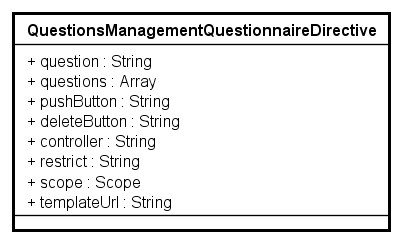
\includegraphics[scale=0.45]{UML/Classi/Front-End/QuizziPedia_Front-end_Controller_QuestionnaireQuestionsManagementController.png}
	\caption{QuizziPedia::Front-End::Controllers::QuestionnaireQuestionsManagementController}
\end{figure} \FloatBarrier
\begin{itemize}
	\item \textbf{Descrizione}: questa classe permette di gestire il recupero delle domande per il questionario;
	\item \textbf{Utilizzo}: fornisce le funzionalità per il recupero delle domande dal back-end e le rende disponibili per poter popolare le view;
	\item \textbf{Relazione con altre classi}:
	\begin{itemize}
		\item \textit{IN} \texttt{QuestionnaireQuestionsManagementDirective}: rappresenta il componente grafico che permette all'utente di:
		\begin{itemize}
			\item Effettuare delle ricerche sul database di domande;
			\item Selezionare le domande da inserire nel questionario;
			\item Mostrare le domande già inserite e permettere all'utente di eliminarle da tale lista.
		\end{itemize}
		Questo componente si presta sia per la creazione che per la modifica di un questionario;
		\item \textit{IN} \texttt{QuestionsService}: questa classe permette di ottenere domande esistenti e salvare nuove domande;
	\end{itemize}
	\item \textbf{Attributi}:
	\begin{itemize}
		\item \texttt{-} \texttt{\$scope: \$scope} \\
		Campo dati contenente un riferimento all’oggetto \$scope creato da \textit{Angular\ped{G}}, viene utilizzato come mezzo di comunicazione tra il controller e la view. Contiene gli oggetti che definiscono il model dell’applicazione;
	\end{itemize}
	\item \textbf{Metodi}:
	\begin{itemize}
		\item 
	\end{itemize}
\end{itemize}

\paragraph{QuizziPedia::Front-End::Controllers::InputToListController}
\begin{figure} [ht]
	\centering
	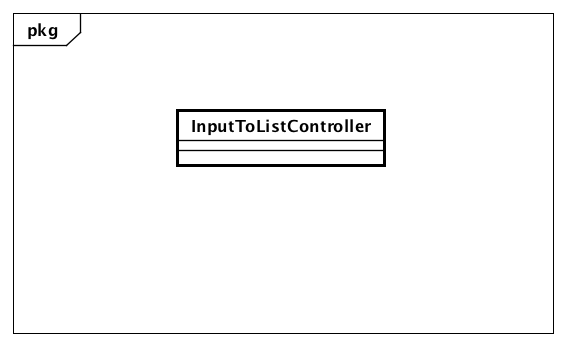
\includegraphics[scale=0.45]{UML/Classi/Front-End/QuizziPedia_Front-end_Controller_InputToListController.png}
	\caption{QuizziPedia::Front-End::Controllers::InputToListController}
\end{figure} \FloatBarrier
\begin{itemize}
	\item \textbf{Descrizione}: questa classe permette di gestire l'inserimento di una lista di risposte durante la creazione di una domanda;
	\item \textbf{Utilizzo}: fornisce le funzionalità per confermare porzioni di domanda durante la creazione;
	\item \textbf{Relazione con altre classi}:
	\begin{itemize}
		\item \textit{IN} \texttt{MultipleQuestionsView}: ;
		\item \textit{IN} \texttt{ConnectionQuestionsModelView}: ;
		\item \textit{IN} \texttt{StringsSortingQuestionsModelView}: ; 
		\item \textit{IN} \texttt{ImagesSortingQuestionsModelView}: ;
	\end{itemize}
	\item \textbf{Attributi}:
	\begin{itemize}
		\item \texttt{-} \texttt{\$scope: \$scope} \\
		Campo dati contenente un riferimento all’oggetto \$scope creato da \textit{Angular\ped{G}}, viene utilizzato come mezzo di comunicazione tra il controller e la view. Contiene gli oggetti che definiscono il model dell’applicazione;
	\end{itemize}
	\item \textbf{Metodi}:
	\begin{itemize}
		\item \texttt{+} \texttt{InputToListController(\$scope: \$scope)}: \\Metodo costruttore della classe.
		\textbf{Parametri}:
		\begin{itemize}
			\item 
		\end{itemize}
		\item \texttt{-} \texttt{putDownAnswer(): void}: \\Metodo che reagisce all'evento di aggiunta nuova risposta e la va a salvare localmente (dobbiamo decidere dove) in modo che venga caricata e visualizzata nella pagina.
	\end{itemize}
\end{itemize}

\paragraph{QuizziPedia::Front-End::Controllers::QuizEventController}
\begin{figure} [ht]
	\centering
	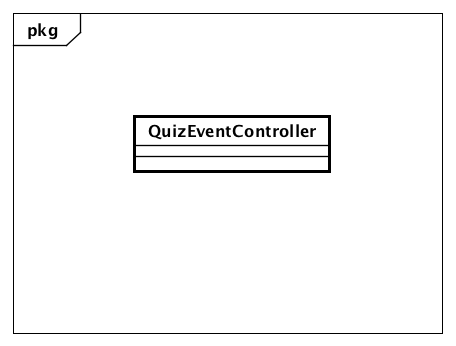
\includegraphics[scale=0.45]{UML/Classi/Front-End/QuizziPedia_Front-end_Controller_QuizEventController.png}
	\caption{QuizziPedia::Front-End::Controllers::QuizEventController}
\end{figure} \FloatBarrier
\begin{itemize}
	\item \textbf{Descrizione}: questa classe permette di reagire ai comandi dell'utente durante la gestione dei suoi questionari;
	\item \textbf{Utilizzo}: fornisce le funzionalità per reagire ai comandi dell'utente, effettua redirect alle pagine richieste, come la visualizzazione delle statistiche di un questionario e iniziare un questionario in modalità esame.
	\item \textbf{Relazione con altre classi}:
	\begin{itemize}
		\item \textit{IN} \texttt{CreationAndModifyDirective}:  
		\item \textit{OUT} \texttt{ExamModalityDirective}:
	\end{itemize}
	\item \textbf{Attributi}:
	\begin{itemize}
		\item \texttt{-} \texttt{\$scope: \$scope} \\
		Campo dati contenente un riferimento all’oggetto \$scope creato da \textit{Angular\ped{G}}, viene utilizzato come mezzo di comunicazione tra il controller e la view. Contiene gli oggetti che definiscono il model dell’applicazione;
	\end{itemize}
	\item \textbf{Metodi}:
	\begin{itemize}
		\item 
	\end{itemize}
\end{itemize}

